% Predlozak za pisanje diplomskog rada na PMF-MO
% Opcenita uputstva za LaTeX se mogu npr. naci na 
% http://web.math.hr/nastava/rp3, http://web.math.hr/nastava/s4-prof/latex.pdf
% NE PREPORUCA se "Ne baš tako kratak uvod u TEX", buduci se radi o vrlo starom prirucniku
% koji nije pogodan za moderne verzije LaTEXa.
% Originalna verzija "The not so short..." na http://tobi.oetiker.ch/lshort/lshort.pdf 
% je obnovljena i daje bolji uvid u moderne verzije LaTeXa

% Stil je optimiziran za kreiranje pdf dokumenta (npr. pomocu pdflatex-a, XeLaTeX-a)

\documentclass[a4paper,twoside,12pt]{memoir} % jednostrano: promijeniti twoside u oneside

% Paket inputenc omogucava direktno unosenje hrvatskih dijakritickih znakova 
% opcija utf8 za unicode (unix, linux, mac)
% opcija cp1250 za windowse
\usepackage[utf8]{inputenc}  % ukoliko se koristi XeLaTeX onda je \usepackage{xunicode}\usepackage{xltxtra}

% Stil za diplomski, unutra je ukljucena podrska za hrvatski jezik
\usepackage{diplomski}
% bibliografija na hrvatskom
\usepackage[languagenames,fixlanguage,croatian]{babelbib} % zahtijeva datoteku croatian.bdf
% hiperlinkovi 
\usepackage[pdftex]{hyperref} % ukoliko se koristi XeLaTeX onda je \usepackage[xetex]{hyperref}

% Odabir familije fontova:
% koristenjem XeLaTeX-a mogu se koristiti svi fontovi instalirani na racunalu, npr
% \defaultfontfeatures{Mapping=tex-text}
% \setmainfont[Ligatures={Common}]{Hoefler Text}
% ili
% \newcommand{\nas}[1]{\fontspec{Adobe Garamond Pro}\fontsize{24pt}{24pt}\color{Chocolate}\selectfont #1}
% i onda \nas{Naslov ...}
\usepackage[pdftex]{graphicx}
\graphicspath{ {images/} }
\usepackage{float}
\usepackage{wrapfig}
\usepackage{url}
\usepackage{lipsum}
\usepackage{hyperref}
\usepackage{cleveref}
\usepackage{epstopdf}
\usepackage{multirow}
\usepackage{caption}
\usepackage[table,usenames,dvipsnames]{xcolor}
\PassOptionsToPackage{hyphens}{url}\usepackage{hyperref}
\usepackage[linesnumbered,ruled,noline]{algorithm2e}
%multi-row
\usepackage{multirow}

\renewcommand*{\listalgorithmcfname}{Lista algoritama}
\renewcommand*{\algorithmcfname}{Algoritam}
\renewcommand*{\algorithmautorefname}{algoritam}

\usepackage{listings}
\definecolor{codegreen}{rgb}{0,0.6,0}
\definecolor{codegray}{rgb}{0.5,0.5,0.5}
\definecolor{codepurple}{rgb}{0.58,0,0.82}
\definecolor{backcolour}{rgb}{0.95,0.95,0.92}

\lstdefinestyle{mystyle}{
	backgroundcolor=\color{backcolour},   
	commentstyle=\color{codegreen},
	keywordstyle=\color{magenta},
	numberstyle=\tiny\color{codegray},
	stringstyle=\color{codepurple},
	basicstyle=\footnotesize,
	breakatwhitespace=false,         
	breaklines=true,                 
	captionpos=b,                    
	keepspaces=true,                 
	numbers=left,                    
	numbersep=5pt,                  
	showspaces=false,                
	showstringspaces=false,
	showtabs=false,                  
	tabsize=2
	}

% Paket graphicx sluzi za manipuliranje grafikom 
 % ukoliko se koristi XeLaTeX onda je \usepackage[xetex]{graphicx}
% Paket amsmath je vec ukljucen
% Dodatno definirane matematicke okoline:
% teorem (okolina: thm), lema (okolina: lem), korolar (okolina: cor),
% propozicija (okolina: prop), definicija (okolina: defn), napomena (okolina: rem),
% slutnja (okolina: conj), primjer (okolina: exa), dokaz (okolina: proof)
% Definirane su naredbe za ispisivanje skupova N, Z, Q, R i C
% Definirane su naredbe za funkcije koje se u hrvatskoj notaciji oznacavaju drukcije 
% nego u americkoj: tg, ctg, ... (\tgh za tangens hiperbolni)
% Takodjer su definirane naredbe za Ker i Im (da bi se razlikovala od naredbe za imaginarni dio kompleksnog
% broja, naredba se zove \slika).
\lstset{
	literate=%
	{ć}{{\'c}}1
	{č}{{\v{c}}}1
	{đ}{{\dj{}}}1
	{š}{{\v{s}}}1
	{ž}{{\v{z}}}1
	{Ć}{{\'C}}1
	{Č}{{\v{C}}}1
	{Đ}{{\DJ{}}}1
	{Š}{{\v{S}}}1
	{Ž}{{\v{Z}}}1
}

\lstloadlanguages{R}
\lstdefinelanguage{Renhanced}[]{R},
	alsoother={:_\$}}
\lstset{ 
	language=R,                     % the language of the code
	basicstyle=\tiny\ttfamily, % the size of the fonts that are used for the code
	numbers=left,                  % where to put the line-numbers
	numberstyle=\tiny\color{codegray},  % the style that is used for the line-numbers
	stepnumber=1,                   % the step between two line-numbers. If it's 1, each line
	% will be numbered
	numbersep=5pt,                  % how far the line-numbers are from the code
	backgroundcolor=\color{white},  % choose the background color. You must add \usepackage{color}
	showspaces=false,               % show spaces adding particular underscores
	showstringspaces=false,         % underline spaces within strings
	showtabs=false,                 % show tabs within strings adding particular underscores
	frame=single,                   % adds a frame around the code
	rulecolor=\color{black},        % if not set, the frame-color may be changed on line-breaks within not-black text (e.g. commens (green here))
	tabsize=2,                      % sets default tabsize to 2 spaces
	captionpos=b,                   % sets the caption-position to bottom
	breaklines=true,                % sets automatic line breaking
	breakatwhitespace=false,        % sets if automatic breaks should only happen at whitespace
	title=\lstname,                 % show the filename of files included with \lstinputlisting;
	% also try caption instead of title
	keywordstyle=\color{blue},      % keyword style
	commentstyle=\color{codegreen},   % comment style
	stringstyle=\color{OliveGreen},      % string literal style
	morekeywords={*,...}            % if you want to add more keywords to the set
} 



\pagestyle{headings}
% uz paket fancyhdr mogu se lako kreirati fancy zaglavlja i podnozja

% Podaci koje treba unijeti
\title{Analiza postupka procjene položaja temeljem
	zadanih pseudoudaljenosti u programski određenom
	prijamniku za satelitsku navigaciju}
\author{Mia Filić}
\advisor{izv. prof. dr. sc Luka Grubišić i prof. dr. sc Renato Filjar}  % obavezno s titulom (prof. dr. sc ili doc. dr. sc.)
\date{\today}  % oblika mjesec, godina

% Moguce je unijeti i posvetu
% Ukoliko nema posvete, dovoljno je iskomentirati/izbrisati sljedeci redak 
\dedication{Na kraju}

\begin{document}

% Naredna frontmatter generira naslovnu stranicu, stranicu za potpise povjerenstva, eventualnu posvetu i sadrzaj
% Moze se iskomentirati ukoliko nije u pitanju konacna verzija
\frontmatter

% Tekst diplomskog ...

%\chapter[Naslov poglavlja u sadržaju][Kratki naslov poglavlja]{Naslov poglavlja}	
% ukoliko naslov nije jako dugacak dovoljno je samo \chapter{Naslov poglavlja} 

%\section[Naslov sekcije u sadržaju][Kratki naslov sekcije]{Naslov sekcije}
%\subsection{Naslov podsekcije}

%\chapter[Globalni navigacijski satelitski sustav (GNSS)][GNSS]{Globalni navigacijski satelitski sustav (engl. Global Navigation Satellite System (GNSS))}
\begin{intro}
Globalni navigacijski satelitski sustav (GNSS) je osmišljen s ciljem da
u bilo kojem trenutku i za bilo koji entitet na Zemljinoj površini može dati podatak
o trenutnom vremenu, položaju i brzini gibanja (engl. Position, Velocity and Time (PVT)). 
Kao takav daje temelje rastućem broju tehnoloških i društveno-ekonomskih sustava.
	\begin{figure}[H]
		\centering
		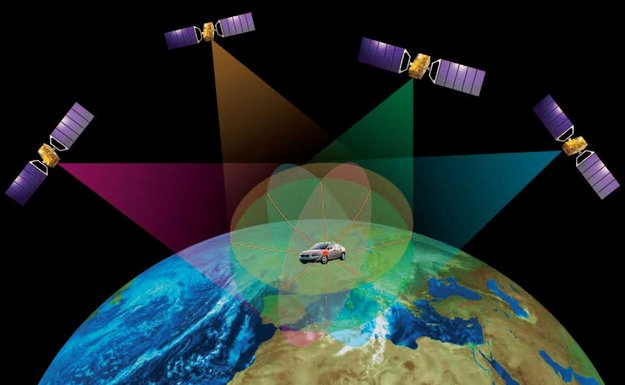
\includegraphics[width=0.6\textwidth]{pictureNav}
		\caption{Satelitska navigacija\cite{bookProcessing} }
		\label{Fig:nn}
		
	\end{figure}
	%http://www.academia.edu/12873735/PRIMJENA_GPS_GLOBALNI_NAVIGACIJSKI_SISTEM_i_GNSS_GLOBALNI_NAVIGACIJSKI_SATELITSKI_SISTEM_U_GEOLO%C5%A0KOM_KARTIRANJU_I_IZRADI_IN%C5%BDENJERSKO-GEOLO%C5%A0KIH_KARATA_NA_PRIMJERU_KLIZI%C5%A0TA_JUNUZOVI%C4%86I_SREBRENIK
	%primjena u kartografiji
	Koristeći pojam GNSS, najčešće se misli na \textit{"sazviježđe"}
	satelita koji odašilju signale potrebne za određivanje trenutne pozicije (i/ili brzine i vremena) i \textit{Navigacijske poruke} (engl. Navigation Messages (NM)).
	\textit{"Sazviježđe"} satelita predstavlja (1) svemirski segment GNSS sustava.
	Postoje još (2) kontrolni segment koji čine kontrolne stanice smještene na Zemlji i (3) korisnički segment, odnosno GNSS prijemnici (Slika \ref{Fig:GNSSsegmenti}).
	Kontrolni segment nadzire i upravljaja radom sustava.
	
	\begin{figure}[H]
			\centering
			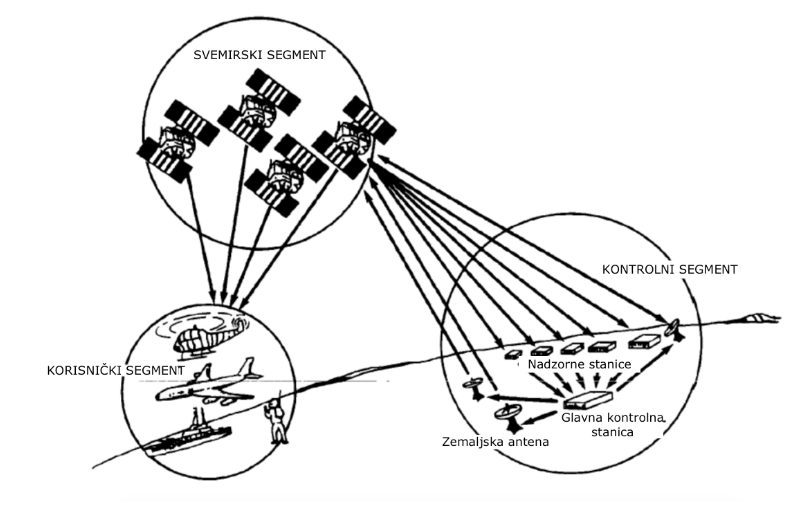
\includegraphics[width=0.6\textwidth]{GNSSsegmenti}
			\caption{Segmenti GNS sustava (GNSS)} %https://dr.nsk.hr/islandora/object/fpz%3A511/datastream/PDF/view
			\label{Fig:GNSSsegmenti}
			
	\end{figure}
	
	Trenutno postoji nekolicina GNS sustava (GNSS). Neki su u potpunosti 
	operativni, dok neki samo djelomično.
	Najraširaniji u civilnoj upotrebi je GPS (Global Positioning System).
	GPS je u potpunosti operativan i u vlasništnu Vlade SAD-a. Njime upravlja Ministarstvo obrane SAD-a (engl. US Air Force).
	GPS omogućava dvije znatno različite razine korištenja, civilnu i vojnu.
	Vojna razina korištenja pruža više mogućnosti, a dopuštena je samo određenim 
	korisnicima. Civilna razina korištenja je dostupna svima, bez dodatne naknade, uz uvjet posjedovanja GPS prijemnika. 
	
	Drugi, također u potpunost operativan GNSS, je GLONASS (Global'naya Navigatsionnaya Sputnikovaya Sistema) u vlasništvu Rusije.
	Neki od GNSS sustava u razvoju su: (1) Galileo i (2) BeiDou.
	Galileo-om upravlja Europska unija (EU). Najavljeno je da će postati u potpunosti operativan do 2020 \cite{bookProcessing}.
	BeiDou je kineski lokalni navigacijski satelitski sustav. U procesu je projekt proširenja BeuDou-a do globalnog do 2020\cite{bookProcessing}.
	
	\begin{table}[H]
		\caption{Obilježja različitih satelitskih navigacijskih sustava}
		%\rowcolors{1}{}{lightgray}
		\begin{center}
			\begin{tabular}{|lllll|}
				\hline
				\rowcolor{lightgray}&  &  & &  \\
				\rowcolor{lightgray}&  &  & &  \\
				 \multirow{-3}{1cm}{ \cellcolor{lightgray}	} & \multirow{-3}{2cm}{\cellcolor{lightgray} Zemlja} & 
				 \multirow{-3}{2cm}{ \cellcolor{lightgray}Broj operativnih satelita} & \multirow{-3}{3cm}{\cellcolor{lightgray} Frekvencije vala nosilaca} & \multirow{-3}{3cm}{\cellcolor{lightgray} Brzina slanja navigacijske poruke} \\
				\hline\hline
				GPS & SAD & 31 & {L1 = 1575.42}
				& 50, 25 \\
				 &  &  & L2 = 1227.60 &  \\
				 &  &  & L5 = 1176.45 &  \\
				\hline
				GLONASS & Rusija & 28 & {L1 = oko 1602}
				& 50 \\
				 &  &  & L2 = 1246 &  \\
				 &  &  &&  \\
				\hline
				Beidou & NR Kina & 22 & {B1 = 1575.42}
				& - \\
				&  &  & B2 = 1191.795 &  \\
				&  &  & B3 = 1268.52 &  \\
				\hline
				Galileo & EU & 18 & {E1 = 1575.42}
				& - \\
				&  &  & E5a-Q = 1176.45 &  \\
				&  &  & E5b-Q = 1207.14 &  \\
				&  & \multirow{-3}{2.5cm}{(15 potpuno operativnih)} & E6 = 1278.75 &  \\
				\hline
			\end{tabular}
		\end{center}
		\label{tab:multicol}
	\end{table}
	
	Primjena GNSS-a dijeli se na pozicioniranje i navigaciju.
	\begin{defn}[Navigacija]
		Navigacija obuhvaća trenutno određivanje položaja i brzine entiteta u pokretu.
		Svrha navigacije je praćenje i upravljanje gibanja entiteta.
	\end{defn}
	
	\begin{defn}[Pozicioniranje]
		Pozicioniranje nazivamo postupak određivanja položaja točkovnog entiteta ili niza 
		točkovnih entiteta u prostoru.
	\end{defn}
	Ovaj rad se bavi isključivo bespojenom (engl. off-line) navigacijskom primjenom, u svrhu praćenja entiteta.
	Bespojena navigacija se koristi u prometnoj znanosti u analizi prometnih puteva. Kako ne zahtjeva izračunavanje u realnom vremenu (engl. real-time),
	svodi se na određivanje položaja točkovnog entiteta koji je statičan u danom vremenu $t$, tj. pozicioniranje.
	Određujući položaj entiteta za niz vremena $ t_1,t_2, \hdots ,t_n $, dobiva se 
	aproksimacija kretanja entiteta u vremenskom okviru $[t_1,t_n]$.
	Preciznost aproksimacije kretanja zadaje se veličinom okvira i parametrom $n$, ili dostupnošću podataka.
	Praksa ne zathjeva da je $n$ u odnosu na vremenski okvir duljine 1 sata prevelik.
	Točno kretanje entiteta moguće je
	odrediti preslikavanjem dobivene aproksimacije na kartu prometnih puteva.
	U tu se svrhu koriste otprije poznati algoritmi.
	Dakle, rad se zasniva na algoritmu za pozicioniranje (statičkog entiteta)
	u konceptu jednog, određenog, GNSS-a: GPS u aspektu civilne razine korištenja.
	
	%TODO sto koje poglvlje donosi
\end{intro}
	
\chapter[Globalni pozicijski sustav (GPS)][GPS]{Globalni pozicijski sustav (GPS, engl. Global Positioning System)}
	Sazvježđe GPS-a se sastoji od najmanje 24 satelita raspoređenih u 6 jednako odmaknutih orbita, svaka s inklanacijom od $55$ stupnjeva od ekvatorijalne
	ravnine (engl. Medium Earth Orbit (MEO)).
	Sateliti kruže na visini od oko 20200 kilometara od Zemljine površine s periodom rotacije 12 zvjezdanih sati. 
	Sateliti su raspoređeni na način da u svakom trenutku za svako mjesto na Zemljinoj površini postoje barem 4 dostupna satelita. Definicija dostupnosti satelita je dana u kasnijem teksu (Stranica \pageref{stranica:dostupnost}).
	
	Svi GPS sateliti odašilju (radio)signale na istoj osnovnoj frekvenciji/frekvencijama (Slika \ref{Fig:GPSSignal}). 
	U satelitima, vrijeme je praćeno pomoću cezijevih satova koji se sinkroniziraju s univerzalnom GPS atomskom vremenskom skalom. Sinkronizacija se odvija u periodima.
	\begin{figure}[H]
		\centering
		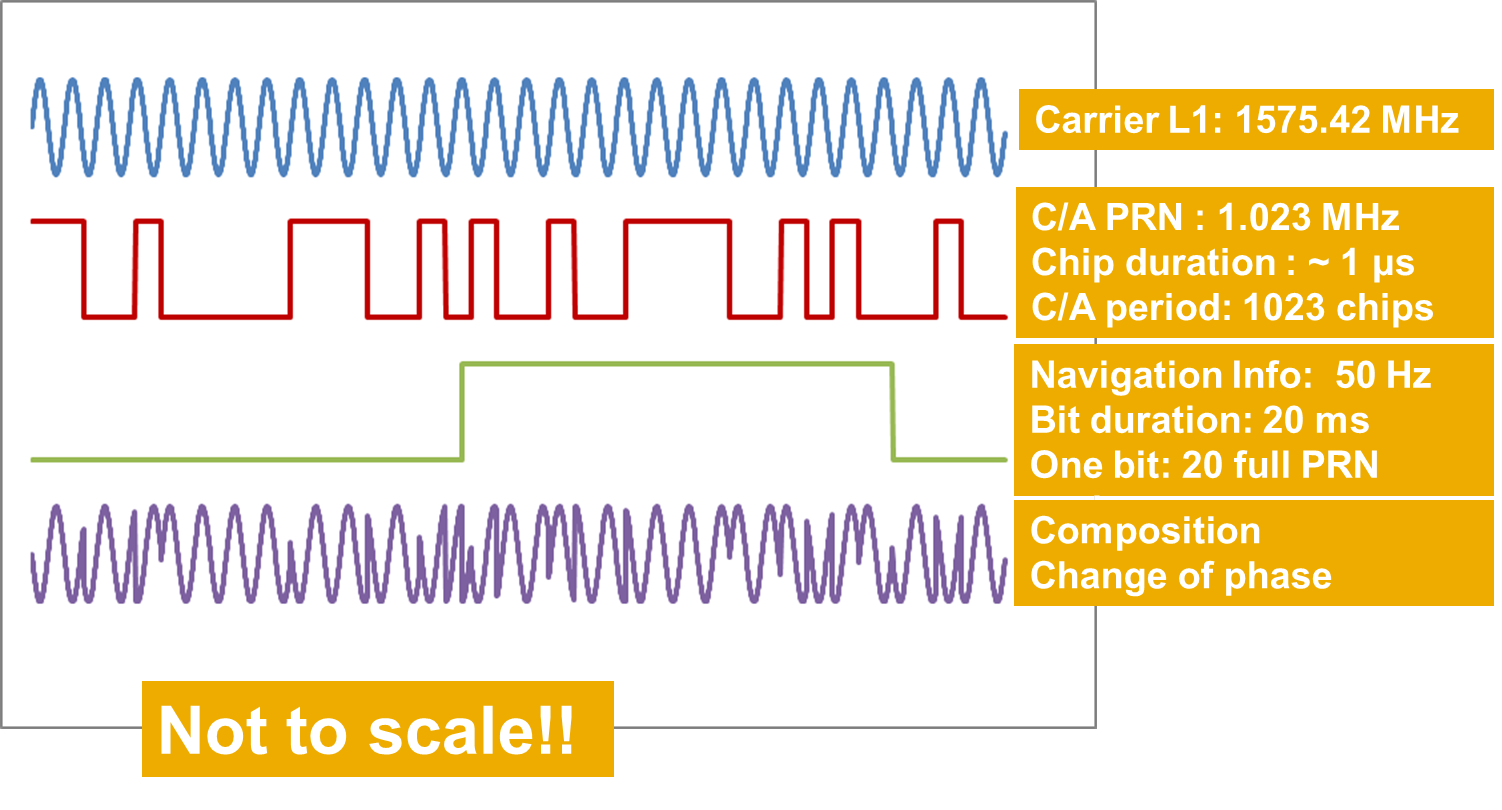
\includegraphics[width=0.4\textwidth]{GPS_Signals}
		\caption{GPS signal i njegove komponente \cite{GPS:1}}
		\label{Fig:GPSSignal}
	\end{figure}
	
	\section[C/A PRN kod]{GPS signali: C/A PRN i P kod}
	\subsection{C/A PRN kod i primjene}\label{CAkod}
	GPS sateliti odašilju signale na dvije frekvencije (nosača) $L_1$ i $L_2$, od kojih je $L_1$ na 1575.42 MHz namjenjena civilnoj upotrebi. Pojam signal se često u satelitskoj navigaciji
	koristi samo za dio GPS signala koja sadržava C/A PRN kod (eng. Coarse Acquisition Pseudo Random Noise). 
	Svaki satelit posjeduje jedinstveni C/A PRN kod koji predstavlja niz 0 i 1 duljine 1023 bit-a.
	GPS-prijemnik razlikuje signale ( signale koji sadrže podatke potrebne za određivanje položaja i \textit{Navigacijske poruke}) različitih satelita
	temeljem sadržanih C/A PRN kodova. Satelit C/A PRN kodove odašilje neprestano, s početkom na početku svake sekunde. Prijemnik primljeni C/A PRN kod korsti za 
	razlikovanje satelita odašiljetelja, ali i za računanje pseudo-udaljenosti.
	
	\begin{defn}[Pseudo-udaljenost]
		Naka su svi sateliti numeriraniprirodnim  brojevima s početkom 
		u 1. Naka je $\mathbf{i} \in \mathbb{N}$ neki satelit i $\mathbf{t}$ prijemnik
		koji je u mogućnosti primiti signal koji odašilje satelit $\mathbf{i}$. Pseudo-udaljenost
		između satelita odašiljatelja $\mathbf{i}$ i prijemnika primatelja $\textbf{t}$:
		$$d_i = c\cdot(t'_i- t_i)$$
		gdje je c konstanta koja je jednaka (prosječnoj) brzini putovanja signala od satelita do prijemnika. $t'_i$ je vrijeme primanja signala, a $t_i$ vrijeme slanja signala
		(po UTC vremenu).
	\end{defn}
	\textbf{Pseudo-udaljenost} je aproksimacija udaljenosti između satelita odašiljatelja i prijemnika primatelja signala u određenom trenutku.
	Neka je $\Delta t := (t'_i- t_i)$. Vrijeme putovanja signala izračunava se poravnavanjem odgovarajućih dijelova signala, tj. C/A PRN kodova.
	Naime, prijemnik i satelit istovremeno generiraju isti C/A PRN kod. Budući da 
	dok signala putuje, prijemnik još uvijek generira C/A PRN kod, po primitku signala,
	ta 2 koda se uspoređuju, poravnavaju. Temeljem razlike u poravnanju, dobivenog i generiranog C/A PRN koda,
	računa se procjena vremena putovanja, tj. $\Delta t$ (Slika \ref{fig:deltat}).
	\begin{figure}[H]
		\centering
		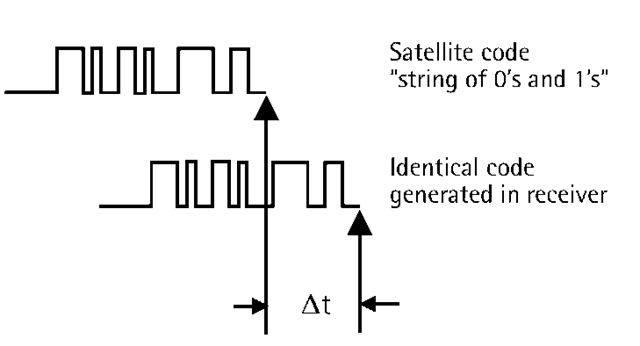
\includegraphics[width=0.4\textwidth]{deltat}
		\caption{Procjena vremena putovanja signala ($\Delta t$)}
		\label{fig:deltat}
	\end{figure}
	Za vrijednost konstante $c$ se uzima brzina svjetlosti koja predstavlja brzinu putovanja poruke satelita u vakuumu. Ona dovoljno dobro modelira stvarnu prosječnu brzinu putovanja.
	
	Budući da se psudo-udaljenost dobiva poravnavanjem kodova\label{stranica:kodno},
	upravo opisani način određivanja pseudo-udaljenosti naziva se kodni.
	
	Postoji još i fazni način određivanja psudo-udaljenosti koji se zasniva na poravnanju valova nosača (engl. Carrier phase) nakon micanjem C/A PRN i P(Y) kodova  iz poruke (Slika \ref{Fig:GPSSignal}).
	Fazno mjerenje služi kao nadopuna kodnom mjerenju u svrhu poboljšanja točnosti određivanja položaja.
	
	
	\section{P kod}\label{Pkod}
	P kod je dio GPS signala koji se odašilje na obje frekvencije i rezerviran je za vojnu razinu upotrebe.
	Kao i C/A PRN kod, sastoji se od niza nula i jedinica i šalje se brzinom 1023 bit/s, ali je znatno dulji.
	Potrebno je ukupno 37 tjedana kako bi se sekvencijalno poslao cjelokupni P kod.
	Za razliku od C/A koda, gdje svaki satelit ima svoj jednistveni C/A kod, P kod je
	distribuiran među satelitima. Isječci P koda koji pripadaju različitim satelitima međusobno su različiti.
	Svakih 7 dana u točno određeno vrijeme određeni satelit odašilje svoj dio P koda.
	Na taj način, prijemnik razlikuje jedan satelit od drugoga. Npr. ukoliko
	satelit $\mathnormal{S}$ odašilje 14. tjedan P koda, onda je satelit $\mathnormal{S}$
	zapravo \textit{Space Vehicle 14 (SV 14)}.
	Kako bi se rezerviralo korištenje P koda samo za vojnu razinu upotrebe,
	prijemnik signalom ne prima goli P kod, već njegovu kriptiranu verziju, u oznaci $P(Y)$.
	Također, samo korisnicima s vojnom razinom upotrebe se prosljeđuje informacija kako dekriptirati $P(Y)$ u $P$.
	$P$ kod omogućava točnije određivanje pozicije entiteta.
	
	\section{Pogreške određivanja položaja i vrste}\label{sec:pogreske}
	Pogreške određivanja položaja se grubo dijele na dvije vrste: (1)
	pogreške nastale usljed konstrukcije ulaza algoritma i
	(2) usljed primjenje algoritma za određivanje položaja na mjerenim psudo-udaljeniostima.
	Dakle, postoje dva izvora: ulazni podatci algoritma (tip 1) i algoritam (tip 2).
	Najčešći izvori pogreške tipa 1 su pogreške pri određivanju pseudo-udaljenosti
	ili raspoređenost satelita oko Zemlje (Slike \ref{fig:DOP}, \ref{fig:DOPLow} i \ref{fig:DOPHigh}).
	Dvije skupine utjecajnih veličina (izvori pogrešaka tipa 1) nazivamo:%
	\begin{itemize}
		\item korisnička razdioba pogrešaka (UERE) i 
		\item geometrijska degradacija točnosti (GDOP).
	\end{itemize}
	Nepovoljan položaj promatranih satelita može rezultirati skoro pa zavisnim jednadžbama
	u \ref{eq:1}.
	\begin{figure}[H]
		\centering
		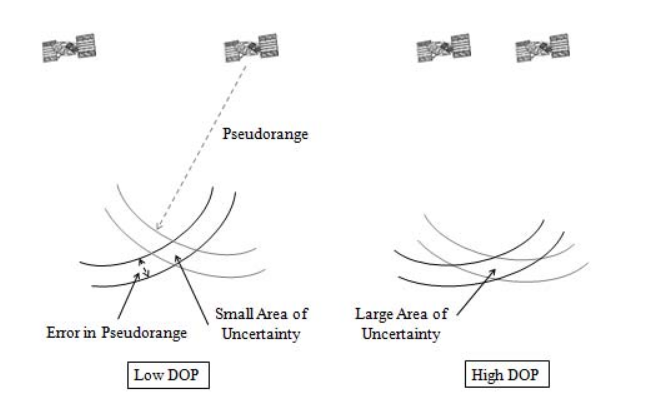
\includegraphics[width=0.6\textwidth]{DOP}
		\caption{Razlike u razmještaju satelita}
		\label{fig:DOP}
	\end{figure}%
	\begin{figure}[H]
		\centering
		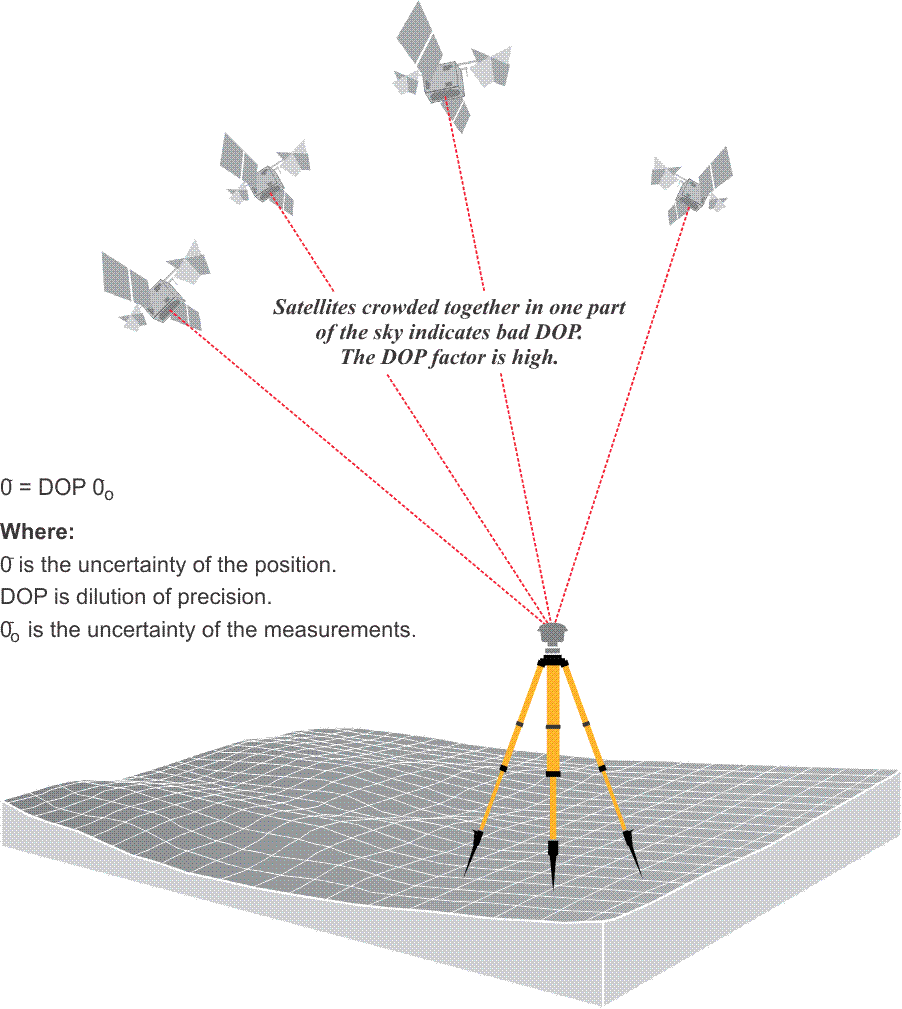
\includegraphics[width=0.6\textwidth]{DOPLow}
		\caption{Nepovoljan razmještaj satelita}
		\label{fig:DOPLow}
	\end{figure}%
	\begin{figure}[H]
		\centering
		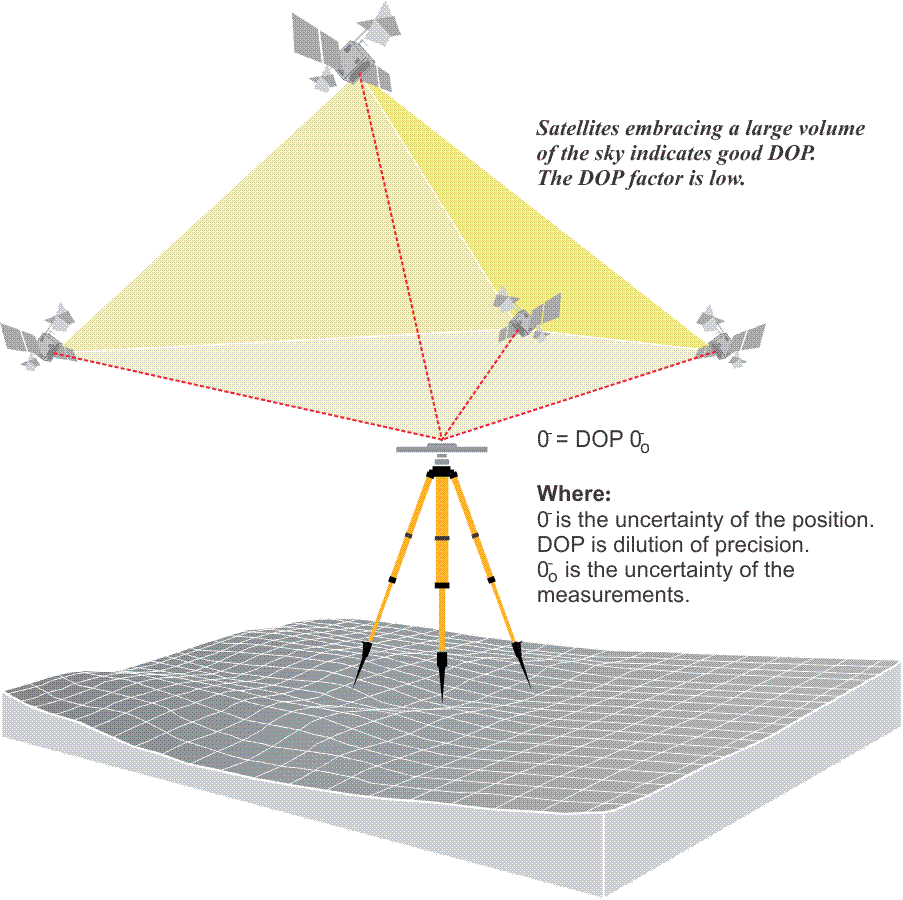
\includegraphics[width=0.4\textwidth]{DOPHigh}
		\caption{Povoljan razmještaj satelita}
		\label{fig:DOPHigh}
	\end{figure}
	
	
	
	Detaljnija podjela pogrešaka tipa 1 nastalih 
	pri određivanju psudo-udaljenosti (UERE pogreške) i područje utjecaja dano je sljedećom tablicom.
	
	\begin{table}[H]\centering
		\caption{Izvori i utjecaj pogreške tipa 1 na određivanje pseudo-udaljenosti}
		\begin{tabular}{ |p{3cm}|p{4cm}| }
			\hline
			\rowcolor{lightgray} Izvor & Utjecaj \\[0.5ex]
			\hline\hline
			\multirow{2}{4em}{satelit} & pogreške orbite  \\ 
			& pogreška sata satelita   \\ 
			\hline
			\multirow{2}{4em}{rasprostiranje signala} & troposferska refrakcija  \\ 
			& ionosferska refrakcija  \\
			\hline
			\multirow{4}{4em}{prijemnik} & pogreške antene  \\ 
			& pogreška sata\\ 
			%OVO je tip 2
			%& pogreška pojednostavljena računalnih
			%postupaka (tip 2)\\
			\cline{2-2}
			& pogreška višestaznih puteva \\
			\hline
		\end{tabular}
	\end{table}	
	
	One mogu biti sistemske ili slučajne. %KOJA JE RAZLIKA?
	Utjecaj sistemskih pogrešaka otklanja se modeliranjem ili
	kombinacijom opažanja.
	Korištenjem više prijemnika, otkanjaju se pogreške spacifične za satelite.
	Pogreške specifične za prijemnike otkanja korištenje viška satelita.
	Utjecajem troposfere je najsigurnije otkloniti modeliranjem,
	a ionosfere korištenjem dva signala različitih frekvencija.
	Nažalost, ponekad nije moguće korištenje dva signala različitih frekvencije
	pa se i utjecaj ionosfere otkanja modeliranjem. Ukoliko se utjecaj ionofere otklanja
	modeliranjem, uvijek ostaje dio slučajne pogreške utjecaja ionosfere
	koja se može uzeti u obzir prilikom izgradnje algoritma za određivanje položaja
	u navigacijskoj domeni (Poglavlje \ref{sec:algTezine}).
	
	Slučajne pogreške nastaju zbog trenutnog mjerenja i slučajnog dijela
	višestruke refleksije signala (multipath) nastalog interferencijom 
	direktnog i reflektiranog signala (Slika \ref{fig:multipath}).
	\begin{figure}[H]
		\centering
		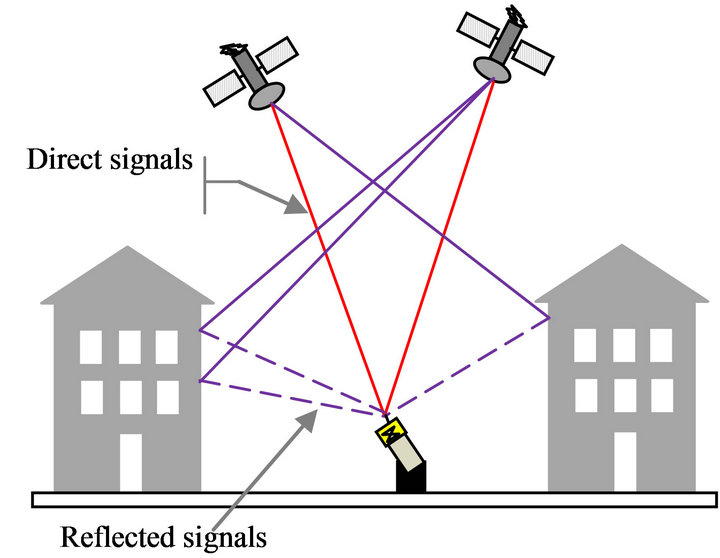
\includegraphics[width=0.4\textwidth]{multipath}
		\caption{Višestruka refleksija signala}
		\label{fig:multipath}
	\end{figure}
	
	U poglavlju \ref{sec:izvedba} prvo se izvodi osnovni algoritam za određivanje položaja 
	prijemnika koji polazi od pretpostavke o potpunoj ispravljenosti pseudo-udaljenosti\label{stranica:greskaOvisisamoOxOpravdano}.
	Kasnije, uvođenjem težina (Poglavlje \ref{sec:algTezine}), reducira se utjecaj pogrešaka
	psudo-udaljenosti.
%	Sistemske pogreške lako se otklanjaju otklonjene koristeći RTK-LIB <- ali ja to modeliram.
%	%RTK LIB u POGLAVLJE 4).
%	 Prije konstrukcije ulaza algoritma za određivanja položaja, smatramo da je
%	pogreška s izvorom u pseudo-udaljenostima maksimalno reducirana.
%	Dakle, pretpostavljamo kako ona više nije značajna
%	neuzimajući ju u obzir u daljnjem postupku izračuna položaja. \label{stranica:greskaOvisisamoOxOpravdano}
%	Smatramo da koristimo potpuno ispravljene pseudo-udaljenosti.
	
	\vspace{0.5cm}
	Pogreške tipa 2 mogu imati izvor u dizajnu izvedbe algoritma ili samoj izvedbi, npr.
	numeričke greške, greške zbog ograničene preciznosti računala,
	aproksimacije pojedinih vrijednosti.
	
	One se ne modeliraju algoritmima procjene položaja (Poglavlje \ref{sec:algoritam}), već prilikom dizajna izvedbe odabranog algoritma (Poglavlje \ref{sec:izvedba})
 	
	%U poglavlju \ref{sec:izvedba}, biti će obrađena analiza pogreške tipa 2 za odabrani algoritam.
	
	\section{Navigation Message}\label{sec:NM} %http://what-when-how.com/gps/gps-details/
	Svaki satelit, uz C/A PRN i P kod, odašilje i dodatne podatke potrebne za ispravo pozicioniranje prijemnika. Odašilje ih u obliku \textit{Navigacijske poruke} koja se šalje zajedno s generiranim C/A PRN kodovima (Slika \ref{Fig:GPSSignal}).
	
	Navigacijska poruka se sastoji od 25 okvira \cite{bookProcessing}.
	Jedan okvir se satoji od 5 podokvira i svaki sadržava vrijeme slanja
	sljedećeg okvira (Slika \cite{GPS:1}). Za slanje cjelokupnog podokvira potrebno je 6 sekundi,
	6 cjelokupnih C/A PRN kodova. Prijemnik je u mogućnosti računati pseudo-udeljenost za novu poziciju satelita svakih
	6 sekundi.
	Za slanje cjelokupne NM, potrebno je 12.5 minuta.
	U nastavku termin poruka koristi se misleći na podprozor.
	\vspace{0.5cm}
	
	Prozor sadrži:
	\begin{enumerate}
		\item GPS vremena odašiljanja,
		\item signal prijenosa s P na C/A kod (potpoglavlja \ref{Pkod} i \ref{CAkod}),
		\item podatke o orbitalnoj putanji satelita,
		\item podatke o korekciji sata satelita,
		\item almanah statusa svih satelita u sazvježđu,
		\item koeficijente preračunavanja GPS vremena u UTC,
		\item ionosferski model korekcije za koji se smatra da je potrebno koristiti.
	\end{enumerate}
	
	\begin{defn}[Universal Time Coordinate (UTC vrijeme)]
		Universal Time Coordinate je vremenski standard zasnovan na međunarodnom atomskom vremenu koji se najčešće koristi u znanstvene i vojne svrhe. Drugi nazivi za taj vremenski standard su ZULU vrijeme i Greenwich Mean Time (GMT).
	\end{defn}
	
	\begin{figure}[H]
		\centering
		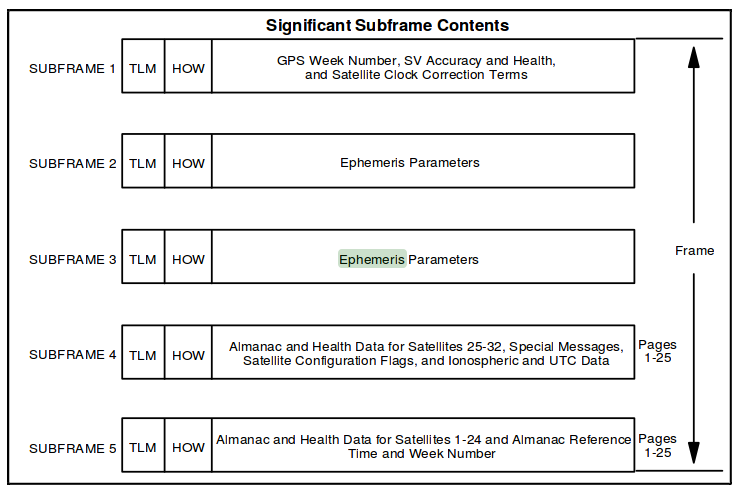
\includegraphics[width=0.6\textwidth]{NACONTENT}
		\caption{Pregled strukture prozora navigacijske poruke\cite{GPS:1}}
		\label{Fig:aaa}
	\end{figure}
	Pojedini dijelovi navigacijske poruke pomažu pri otklanjaju pogrešaka tipa 1  
	(Potpoglavlje \ref{sec:pogreske}), određivanju
	pseudo-udaljenosti i trenutnoj poziciji satelita.
	Naime, iz podataka o orbitalnoj putanji satelita moguće je za odabrani trenutak izračunati poziciju (koordinate) satelita u orbitalnom koordinatnom sustavu pa i svakom drugom.
	 
	Za razumjevanje ovoga rada, dovoljno je razumjeti sljedeće.
	Prijemnik svakih 6 sekundi ima dovoljno podataka da odredi novu pseudo-udaljenost do istog satelita sve dok on ne prestane biti dostupan. 
	
	\begin{defn}[Dostupnost satelita $\mathnormal{S}$ prijemniku $\mathnormal{T}$]
		\label{stranica:dostupnost}
		Za satelit $\mathnormal{S}$ kažemo da je dostupan prijemniku $\mathnormal{T}$ u trenutku $\mathnormal{t}$ ako je u sljedećih 6 sekundi u mogućnosti izračunati
		pseudo-udaljenost do satelita $\mathnormal{S}$ i konstruirati sljedeću jednadžbu:
		\begin{align}\label{eq:position1}
		d_s = \sqrt{(x-x_s)^{2}+(y-y_s)^{2}+(z-z_s)^{2}}
		\end{align}
		gdje su jedine nepoznanice $(x,y,z)$, tj. koordinate položaja prijemnika.
		$(x_s,y_s,z_s)$ su koordinate položaja satelita. 
	\end{defn}
	
	\section{Proces određivanja položaja}\label{sec:positionProcess}
	U pravilu, u svakom trenutku, prijemnik ima više dostupnih satelita od kojih dobiva poruke. Za određivanje položaja prijemnika u granicama dopuštene točnosti,
	zahtjevaju se barem 4 dostupna satelita\label{stranica:4satelita}.
	
	Kako bi prijemnik odredio svoju poziciju računa tri nepoznanice: geografsku širinu, duljinu i nadmorsku visinu.
	% odnosno koordinate u trodimenzionalnom pravokutnom koordinatnom sustavu (geoprostornom koordinatnom sustavu) \textit{WGS84}.
	% Geoprostornom koordinatni sustav \textit{WGS84} pred
	
	Neka je $k$ broj vidljivih satelita od prijemnika $\mathnormal{T}$.
	Prijemnik $\mathnormal{T}$ promatrajući poruke dobivene od samo jednog satelita,
	u vremenu $\mathnormal{t}$, izračunava samo jednu pseudo-udaljenost i može konstruirati samo jednu jednadžbu \ref{eq:position1}
	 koja mu omogućava odrediti sferu oko promatranog satelita na kojoj bi se mogao nalaziti (Slika \ref{Fig:1SatelitePosition}).
	
	\begin{figure}[H]
		\centering
		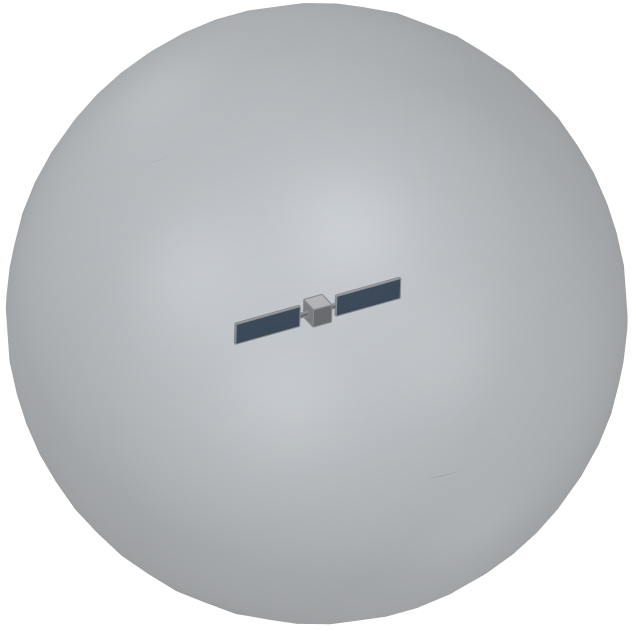
\includegraphics[width=0.4\textwidth]{satellite_distance_13D}
		\caption{Sfera oko promatranog satelita na kojoj bi se prijemnik mogao nalaziti \cite{gps:2}}
		\label{Fig:1SatelitePosition}
	\end{figure}
	Uključujući u izračun pridobivene pseudo-udaljenosti još jednog satelita dobivamo situaciju prikazanu na Slici \ref{Fig:2SatelitePosition}.
	\begin{figure}[H]
		\centering
		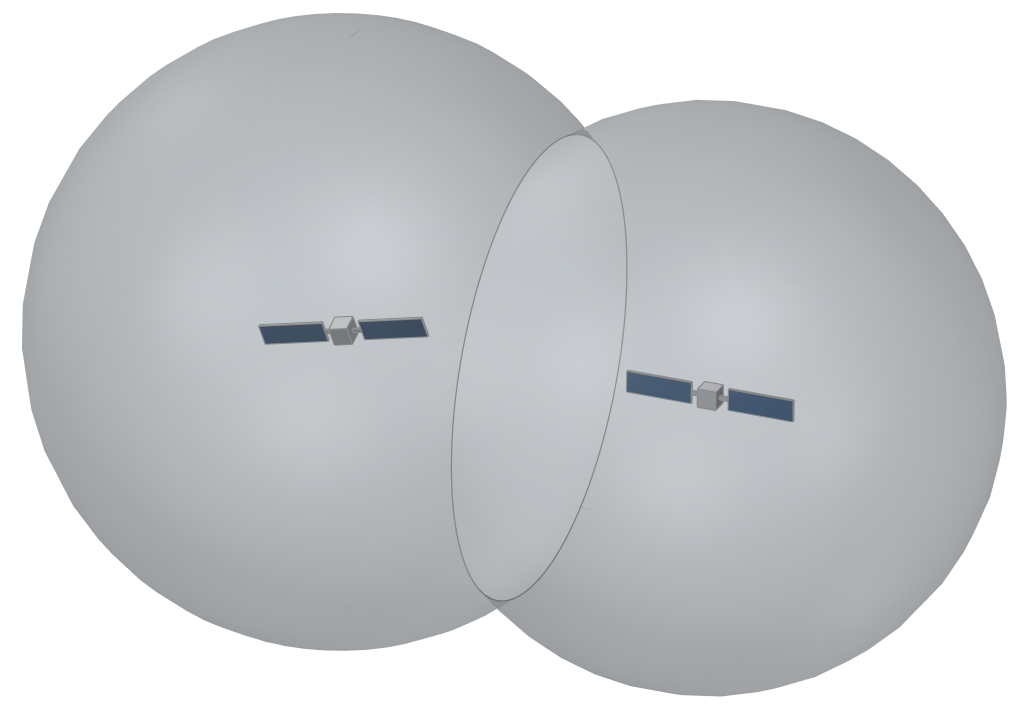
\includegraphics[width=0.6\textwidth]{satellites_distance_23D}
		\caption{Sfere oko dva promatrana satelita. Presjek je kružnica na kojoj bi se prijemnik mogao nalaziti. \cite{gps:2}}
		\label{Fig:2SatelitePosition}
	\end{figure}
	Uključujuči u izračun još jedan satelit, dobivamo situaciju prikazanu na Slici \ref{Fig:3SatelitePosition}.
	
	\begin{figure}[H]
		\centering
		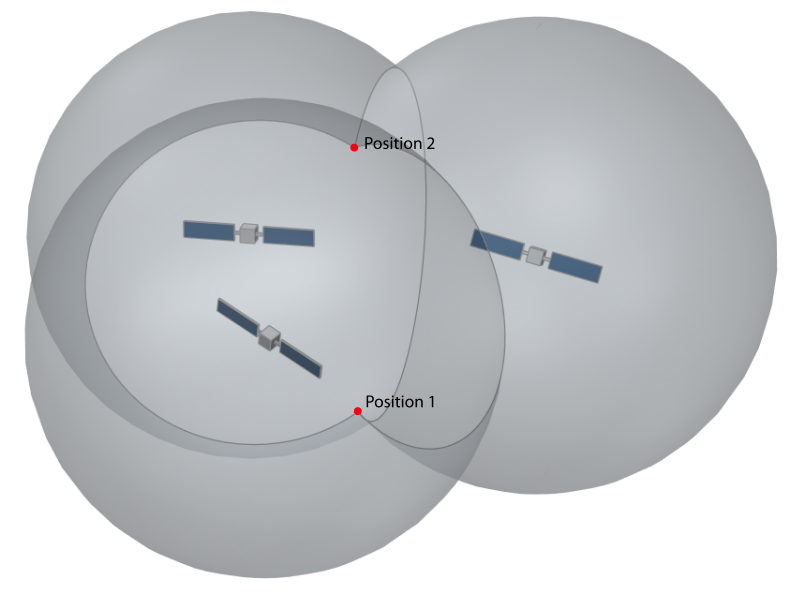
\includegraphics[width=0.6\textwidth]{satellites_distance_33D}
		\caption{Sfere oko tri promatrana satelita. Presjek su dvije točke na kojoj bi se prijemnik mogao nalaziti. \cite{gps:2}}
		\label{Fig:3SatelitePosition}
	\end{figure}
	
	Presjek tri promatrane sfere su dvije točke na kojoj bi se prijemnik mogao nalaziti.
	Jedna točka se nalazi daleko u svemiru, dok je druga točka točka kandidat pozicije prijemnika. 
	
	Algebarski, rješavamo sljedeći sustav linearnih jednadžbi u $(x,y,z)$ :
	\begin{align}\label{eq:position2}
	 d_1 = \sqrt{(x-x_1)^{2}+(y-y_1)^{2}+(z-z_1)^{2}} \notag \\
	 d_2 = \sqrt{(x-x_2)^{2}+(y-y_2)^{2}+(z-z_2)^{2}} \\
	 d_3 = \sqrt{(x-x_3)^{2}+(y-y_3)^{2}+(z-z_3)^{2}} \notag
	\end{align}
	gdje su $1,2 \text{ i }3$,  3 različita satelita, a $(x_i,y_i,z_i)$ pripadajuće
	koordinate položaja satelita u (ECEF XYZ) koordinatnom sustavu.
	ECEF XYZ koordinatni sustav je prikazan na Slici \ref{Fig:na}. Ishodište (ECEF XYZ) koordinatnog sustava je središte zemlje.
	
	\begin{figure}[H]
		\centering
		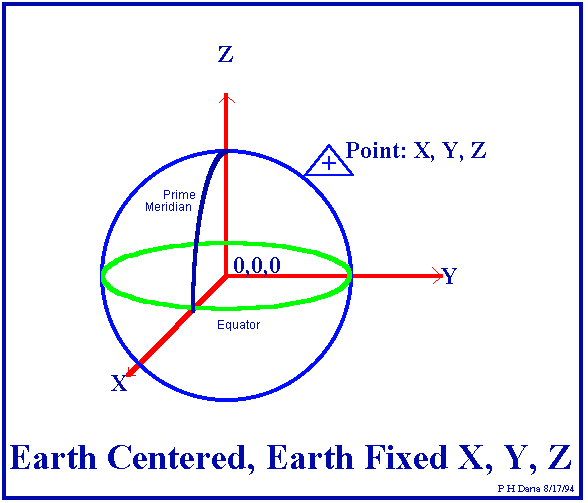
\includegraphics[width=0.6\textwidth]{ecefxyz.png}
		\caption{Earth-Centered, Earth-Fixed $\mathnormal{X}$, $\mathnormal{Y}$, $\mathnormal{Z}$ coordinate system ( ECEF XYZ koordinatni sustav ) \cite{GPS:overview}}
		\label{Fig:na}
	\end{figure}
	
	Svaki prijemnik je sposoban izvesti konverziju iz i u koordinata u ECEF XYZ sustavu 
	u i iz geografskih (geografska širina, duljina i nadmorska visina) \cite{GPS:overview}.
	Dakle, prijemniku su potrebna barem 3 dostupna satelita kako bi odredio poziciju.
	Ali se ipak na stranici \pageref{stranica:4satelita} se postavlja zahtjev na barem 4. 
	
	Primjetimo kako proces određivanja položaja prijemnika
	indirektno zahtjeva usklađenost satova prijemnika i dostupnih satelita.
	Satovi svih satelita su međusobno usklađeni usklađenošću s GPS vremenom. Ukoliko odstupanje ipak postoji, biti će zapisano u navigacijskoj poruci pa se može uzeti u obzir prilikom određivanja položaja prijemnika.
	Napomenimo, GPS vrijeme nije jednako UTC vremenu. GPS vrijeme je bilo 0 u 06.01.1980. i određeno je protjecanjem vremena u GPS satelitima, tj. njihovim 
	satovima. 
	
	Satovi prijemnika nisu iste preciznosti kao satovi satelita.
	Prijemnici obično koriste satove preciznosti do otprilike $10^{-6}$ sekundi.
	Pogreška određivanja vremena od $10^{-6}$ sekundi dovodi do pogreške u
	određivanju pseudo-udaljenosti od oko 300 metara.
	Uključijući u izračin i pogrešku sata prijemnika, pseudo-udaljenost modeliramo jednadžbom:
	$$d_i = c\times(t'_i- t_i+ d_T)$$
	gdje $d_T$ predstavlja spomenutu pogrešku.
	Budući da se prilikom određivanja položaja, 
	spomenuta pogreška u oznaci $d_T$ ne mijenja u odnosu na satelit koji se promatra,
	može se izračunati dodavajući ju kao nepoznanicu u sustav jednadžbi \ref{eq:position2}
	Dakle, sustav jednadžbi \ref{eq:position2} prelazi u:
	\begin{align}\label{eq:position3}
	d_1 = \sqrt{(x-x_1)^{2}+(y-y_1)^{2}+(z-z_1)^{2}} + c\cdot d_T \notag \\
	d_2 = \sqrt{(x-x_2)^{2}+(y-y_2)^{2}+(z-z_2)^{2}} + c\cdot d_T  \\
	d_3 = \sqrt{(x-x_3)^{2}+(y-y_3)^{2}+(z-z_3)^{2}} + c\cdot d_T \notag 
	\end{align}
	
	Kako bi za gornji sustav postojala mogućnost pronalaska rješenja,
	uvodi se zahtjev na još barem jedan dostupni satelit, što je ukupno 4 (Stranica \pageref{stranica:4satelita}).
	Dobivamo sljedeći sustav jednadžbi u $(x,y,z,d_T)$:
	\begin{align}\label{eq:1}
	 d_1 = \sqrt{(x-x_1)^{2}+(y-y_1)^{2}+(z-z_1)^{2}} + c\cdot d_T \notag \\
	 d_2 = \sqrt{(x-x_2)^{2}+(y-y_2)^{2}+(z-z_2)^{2}} + c\cdot d_T  \\
	 d_3 = \sqrt{(x-x_3)^{2}+(y-y_3)^{2}+(z-z_3)^{2}} + c\cdot d_T \notag \\
	 d_4 = \sqrt{(x-x_4)^{2}+(y-y_4)^{2}+(z-z_4)^{2}} + c\cdot d_T \notag
	\end{align}
	
	Upravo opisanom postupkom otklanjamo pogrešku nastalu prilikom 
	određivanja pseudo-udaljenosti 
	s izvorom u pogrešci sata prijemnika.
	U praksi se može koristiti još veći broj dostupnih satelita što poboljšava 
	preciznost pozicioniranja prijemnika. Očekivana pogreška rješenja dobivenog rješavanjem sustava\ref{eq:1} je između $10^2$ i $10^3$. Tako dobiveno rješenje se profinjuje čime se postiže pogreška veličine $10^1$.
	Ovim radom se proučava, opisuje, dizajnira i izvodi algoritam za rješavanje sustava \ref{eq:1}.
	Naime, rješavanje sustava \ref{eq:1} čini temelj procesa određivanja položaja i nužno ga je provesti.
	U primjenama koje zahtjevaju relativno malu točnost, ono je i dovoljno.\\
	Metode za profinjavanje dobivenog rješenja (modeli ispravka) mogu biti izrazito kompleksne i ovise o primjeni. Svojom kompleksnošću i raznovrsnošću prelaze obim ovoga rada.\\

\chapter[Algoritam procjene položaja (APP)]{Algoritam procjene položaja u domeni navigacijske primjene}\label{sec:algoritam}
%Algoritam procjene položaja za ulazne podatke, ne mora nužno određivati nadmorsku visinu, geografsku širinu i duljinu. Postoji više geoprostornih koordinatnih sustava za određivanje
%pozicije objekta. Korištenje nadmorske visine, geografske širine i duljine predstavlja jedan geoprostorni koordinatni sustav. Ovisno o geoprostornom sustavu koordinata korištenih satelita, algoritam određuje geoprostorni koordinatni sustav u kojem će biti prikazana izračunata pozicija prijemnika. 
Ukratko, postupak procjene položaja satelitskim navigacijskim sustavom traži ispunjavanje sljedećih preduvjeta:
\begin{itemize}
	\item Korištenje zajedničkog (geoprostornog) referentnog sustava,
	\item Korištenje zajedničkog vremena (vremenskog okvira) sustava,
	\item Ispunjavanje pretpostavke o pravocrtnom širenju satelitskih signala jedinstvenom
	brzinom (brzina svjetlosti u vakuumu).
\end{itemize}
Uvjeti trebaju biti ispunjeni od strane svih satelita odabranog sustava i korištenog prijemnika.
Prvi uvijet je uvijek lako ispuniti. Druga dva se ispunjavaju na razne načine:
(1) modeliranjem prije primjene algoritma za određivanje položaja u navigacijskoj domeni, (2)
korištenjem viška satelita ili prijemnika, (3) modeliranjem prilikom primjene algoritma za određivanje položaja u navigacijskoj domeni (samim algoritmom), (4) modeliranjem nakon primjene algoritma za određivanje položaja u navigacijskoj domeni.
Na primjer, odstupanje sata prijemnika od vremenskog okvira sustava modelira se kao četvrta nepoznanica sustava 
(Poglavlje \ref{sec:positionProcess}).

\textit{Algoritam procjene položaja u domeni navigacijske primjene} (APP)
smatramo svakim algoritmom koji za sustav jednadžbi \ref{eq:1}
određuje nepoznatu poziciju prijemnika u koordinatama $(x,y,z)$.
Broj jednadži sustava može biti i veći od 4. Tada govorimo o prezasićenim sustavima.
Ovisno o odabiru, APP se može temeljiti na rješavanju sustava nelinearnih jednadžbi pronalaženjem rješenja pomoću (1) metode najmanjih kvadrata (Newton-ova metoda),
(2) metode zatvorene forme, (3) metode najbližeg susjeda \cite{math:positioning}. 

Općenito, rješava se moduficiran sustav jednadžbi \ref{eq:1} uz $d = c \cdot d_T$:\\
\begin{align}\label{eq:new}
d_1 = \sqrt{(x-x_1)^{2}+(y-y_1)^{2}+(z-z_1)^{2}} +d + v_1\notag \\
d_2 = \sqrt{(x-x_2)^{2}+(y-y_2)^{2}+(z-z_2)^{2}} +d + v_2 \\
d_3 = \sqrt{(x-x_3)^{2}+(y-y_3)^{2}+(z-z_3)^{2}} +d + v_3\notag \\
d_4 = \sqrt{(x-x_4)^{2}+(y-y_4)^{2}+(z-z_4)^{2}} +d + v_4\notag
\end{align}
u koji uključejemo nepoznati parametar $(v_1,v_2,v_3,v_4)$, dodatnu pogreška
izračuna.

Uz oznake 
\begin{align}
\mathbf{\rho} := (d_1, d_2, d_3, d_4)^T \\ 
\mathbf{x} := (x,y,z,d_T)^T \\ 
\mathbf{s}_i := (x_i,y_i,z_i)^T \\ 
\mathbf{h} (\mathbf{x}) := 
\begin{bmatrix}
||(s_1-\mathbf{x}_{1:3})|| + x_4\cdot c\\
||(s_2-\mathbf{x}_{1:3})|| + x_4\cdot c\\
||(s_3-\mathbf{x}_{1:3})|| + x_4\cdot c\\
||(s_4-\mathbf{x}_{1:3})|| + x_4\cdot c
\end{bmatrix} \\
\mathbf{v} := (v_i,v_2,v_3,v_4)^T \label{eq:v}
\end{align}%
prelazi u
\begin{align}\label{eq:matrix}
\mathbf{\rho} = \mathbf{h}(\mathbf{x})+\mathbf{v}
\end{align}%
\section{Iterativna metoda najmanjih kvadrata}

Primjetimo kako je $\mathbf{h}(\mathbf{x})$ jednako pravom vektoru pseudo-udaljenosti (udaljenosti, ako pogreška sata, $d_T$ = 0) između
satelita i prijemnika za prave vrijednosti $\mathbf{x}$, $\bar{\mathbf{x}}$.\\

%POPRAVITI, POGLEDAJ IZVOS S PREBACIVANJEM Cd_T i kvadriranjem
Opće dizajniranje algoritma za određivanje položaja u domeni navigacijske primjene nema utjecaj na
pogreške tipa 2,
već samo pogreške tipa 1 (Stranica \pageref{stranica:greskaOvisisamoOxOpravdano}).
Također, pretpostavlja se kako su otklonjene sve pogreške tipa 1 koje imaju izvor 
u pogreškama izračuna pseudo-udaljenosti (osim pogreški sata prijemnika) (Stranica \pageref{stranica:greskaOvisisamoOxOpravdano}).
Ostaje još samo modelirati pogreške koje imaju za izvor trenutni položaj satelita dostupnih za
izračunavanje željenog položaja $\bar{\mathbf{x}}_{(1:3)}$.
U tu svrhu modeliramo vektor pogrešaka $\mathbf{v}$, funkcijom $\mathbf{p}(\mathbf{x})$ koja ovisi o nepoznatom parametru $\mathbf{x}$.
Uz oznaku $\mathbf{y} := \rho$, 
 jednadžba  \ref{eq:matrix} prelazi u
\begin{align}\label{eq:matrix2}
\mathbf{y} = \mathbf{\rho} = \mathbf{h}(\mathbf{x})+ \mathbf{p}(\mathbf{x})
\end{align}%
Preciznije,
član $\mathbf{p}(\mathbf{x})$ modelira pogrešku razlike u procjeni parametra $\mathbf{x}$ od stvarne vrijednosti.
Što je aproksimacija potrebnih vrijednosti za izračun rješenja matrične jednadžbe
\ref{eq:matrix} točnija, to je $\mathbf{p}(\mathbf{x})$ 
bliže nuli za pravu vrijednost $\bar{\mathbf{x}}$.
Aproksimaciju za $\bar{\mathbf{x}}$, u oznaci $\hat{\mathbf{x}}$, pronalazimo tražeći nultočke funkcije $\mathbf{p}(\mathbf{x})$.
U praksi je uobičajeno da mjerenja sadrže pogreške i tada $\mathbf{p}(\mathbf{x})$ uopće ne mora imati 
nultočke i $\hat{\mathbf{x}}$ ne možemo pronaći tražeći nultočke funkcije $\mathbf{p}(\mathbf{x})$.

Ideja metode najmanjih kvadrata je pronalazak $\hat{\mathbf{x}}$ tražeći minimum $\mathbf{p}(\mathbf{x})$, tj.
\begin{align}\label{eq:minimization}
	\hat{\mathbf{x}} = \text{arg min}_\mathbf{x} \mathbf{p}(\mathbf{x})^T\mathbf{p}(\mathbf{x})
\end{align}
Problem opisan jednadžbom \ref{eq:minimization} nije linearan pa
ne postoji općeniti način pronalaska njegovog rješenja.

U slučaju kada su funkcija koju treba minimiziati i početna vrijednost $\mathbf{x}_0$
(iterativnog postupka) dovoljno dobre (vidi: dodatak \ref{appendix:aTay}), rješenja problema \ref{eq:minimization} možemo
dobiti iterativnim postupakom.
Ideja iterativnog postupka je počevši s $\mathbf{x}_0$ računati $\mathbf{x}_1, \mathbf{x}_2, \hdots $ sve dok se novoizračunate vrijednosti ne prestanu mijenjati ili postanu dovoljno bliske prethodnoj, tj.
$\left \| x_{k} - \mathbf{x}_{k-1}\right\| < \delta$ za dovoljno male $\delta > 0$.
$\delta$ još nazivamo i zaustavni kriterij.

Jedan iterativni postupak rješavanja problema \ref{eq:minimization} je Newton-Gaussova metoda (iterativna metoda najmanjih kvadrata).
Newton-Gaussova metoda linearizira $\mathbf{p}(\mathbf{x})$ u okolini od $\mathbf{x_k}$ pomoću prvog člana razvoja funkcije u Taylorov red\label{stranica:NGLin} u točki $\mathbf{x}_k$:
\begin{align}\label{eq:approx}
	\mathbf{p}(\mathbf{x_k}+ \Delta \mathbf{x_k}) \approx \mathbf{p}(\mathbf{x_k}) + \mathbf{p}'(\mathbf{ x_k})\cdot \Delta \mathbf{x_k}
\end{align}

$\Delta \mathbf{x_k}$ se odabire na način tako da
$$lim_{k \to \infty} \left( \mathbf{p}(\mathbf{x_k}) \right) = 0$$ 
jer za pravu vrijednost $\mathbf{x}$ izraz $\mathbf{p}(\mathbf{x}) = 0$ ili poprima svoj minimum ukoliko postoje pogreške
točnosti vrijednosti koje se koriste prilikom konstrukcije sustava.
 
Sada, za $\mathbf{p}(\mathbf{x_{k+1}}) := \mathbf{p}(\mathbf{x_k}+ \Delta \mathbf{x_k}) \approx \mathbf{p}(\mathbf{x_k}) + \mathbf{p}'(\mathbf{x_k})\cdot \Delta \mathbf{x_k}$ želimo
 da je što bliže 0.
 Dakle, $ \Delta \mathbf{x_k} $ odabiremo trežeći minimum funkcije
\begin{align}\label{eq:minDelta}
	\mathbf{p}(\mathbf{x_k}) + \mathbf{p}'(\mathbf{x_k})\cdot \Delta \mathbf{x_k}
\end{align}
u $\Delta \mathbf{x_k}$.

Označimo sada s $J_k := \mathbf{p}'(\mathbf{x_k}) = \mathbf{h}'(\mathbf{x_k})$.
\ref{eq:minDelta} prelazi u 
\begin{align}\label{eq:minDelta2}
	J_k \Delta \mathbf{x_k} +\mathbf{p}(\mathbf{x_k})
\end{align}
čij je minimun dan s (Stranica \pageref{stranica:nastavakLS})  
\begin{align}\label{eq:minDeltaRj}
\Delta \mathbf{x_k} = - (J_k^TJ_k)^{-1}J_k^T \mathbf{p}(\mathbf{x_k})
\end{align}
Izraz za $\mathbf{x_{k+1}}$ je sljedeći:
\begin{align}\label{eq:iter}
	\mathbf{x_{k+1}} = \mathbf{x_{k}} - (J_k^TJ_k)^{-1}J_k^T \mathbf{p}(\mathbf{x_k})
\end{align}
Prilikom izvedbe algoritma, potrebano je pametno odrediti početnu vijednost $\mathbf{x_0}$, te kasnije iterirati po formuli \ref{eq:iter}.
Ukoliko odaberemo dovoljno dobar $\mathbf{x}_0$, dovoljno blizu rješenju i
ako je druga derivacija od $p$ u točki $\bar{\mathbf{x}}$ dovoljno mala,
niz $x_0,x_2, \hdots$ konvergira prema $\bar{\mathbf{x}}$. Izračun $J_k$ za idealan slučaj $d = 0$ se može naći u prilogu \ref{appendix:aTay}.

Algoritam iterativne metode najmanjih je dan u nastavku.

\begin{algorithm}[H]
	\KwData{ $\mathbf{p(\mathbf{x})}, \mathbf{x}_0, \delta$ }
	\KwResult{ $\hat{\mathbf{x}} $ }
	$k = 0$ \;
	\While{$ \left \| \mathbf{x}_{k} - \mathbf{x}_{k-1}\right\| \geq \delta $}{
		$J_k = \mathbf{p}'(\mathbf{x}_k)$ \;
		$\Delta \mathbf{x}_k = - J_k^{-1} \cdot \mathbf{p}(\mathbf{x}_k) $ \;
		$\mathbf{x}_{k+1} =\mathbf{x}_k + \Delta \mathbf{x}_k$ \;
	$k ++$\;
	} 
	$\hat{\mathbf{x}} = \mathbf{x_k}$
\caption{Iterativna metoda najmanjih kvadrata}
\label{code:iterLSM}
\end{algorithm}

Prilikom korištenja gornjeg algoritma za određivanje pozicije entiteta, za $\mathbf{x}_0$ se mogu uzeti koordinate središta zemlje jer su jednadžbe za određivanje položaja dovoljno bliske linearnima.

Ako je poznato da su vrijednosti koje koristimo za konstrukciju
jednadžbi za određivanje položaja \ref{eq:1} za pojedine jednadžbe točnije,
pametno je dati prednost tim jednadžbama pred ostalima.
Važnost pojedine jednadžbe simuliramo pridavanjem težina pojedinoj jednadžbi.
Jednadžbi se pridružuje težina $\sigma_i$ koja je proporcionalna preciznosti 
vrijednosti korištenih prilikom njezine konstrukcije.
Najčešće način pronalaženja odgovarajućih težina je
korištenjem kovarijancone matrice
vektora pogrešaka $\mathbf{v}$ (Jednadžba \ref{eq:v}),u oznaci $\Sigma : = cov(\mathbf{v})$. Minimizacijski problem \ref{eq:minimization} prelazi u %
\begin{align}\label{eq:minimisation2}
\hat{\mathbf{x}} = \text{arg min}_\mathbf{x} \mathbf{p}(\mathbf{x})^T \Sigma^{-1} \mathbf{p}(\mathbf{x})
\end{align}%
Sada, algoritam \ref{code:iterLSM} prelazi u algoritam \ref{code:iterLSMW}.

\begin{algorithm}[H]
	\KwData{ $\mathbf{p(\mathbf{x})}, \mathbf{x}_0, \delta$, $\Sigma$ }
	\KwResult{ $\hat{\mathbf{x}} $ }
	$k = 0$ \;
	\While{$ \left \| \mathbf{x}_{k} - \mathbf{x}_{k-1}\right\| \geq \delta $}{
		$J_k = \mathbf{p}'(\mathbf{x}_k)$ \;
		$\Delta \mathbf{x}_k = - (\Sigma^{-\frac{1}{2}}J_k ) ^{-1} ( \Sigma^{-\frac{1}{2}}(\mathbf{p}(\mathbf{x}_k))$ \;
		$\mathbf{x}_{k+1} =\mathbf{x}_k + \Delta \mathbf{x}_k$ \;
		$k ++$\;
	} 
	$\hat{\mathbf{x}} = \mathbf{x_k}$
	\caption{Iterativna metoda težinskih najmanjih kvadrata}
	\label{code:iterLSMW}
\end{algorithm}
Procjenitelj za $\bar{\mathbf{x}}$ dobiven težinskom metodom najmanjih kvadrata, jednakost \ref{eq:minimisation2}, ima najmanju varijancu među svim procjeniteljima za
$\bar{\mathbf{x}}$. Ukoliko je vektor pogrešaka $\mathbf{v}$ normalno
distribuiran, procjenitelj \ref{eq:minimisation2} postaje procjenitelj
metode najbližeg susjeda (Podpoglavlje \ref{sec:MLE} i MLE procjenitelj).

Prilikom korištenja iterativne metode najmanjih kvadrata potrebno je
modelirati distribuciju vektora pogrešaka, točnije kovarijanconu matricu $\Sigma$.
Također, potrebno je pripazati na 
velike pogreške u određivanju vrijednosti pomoći kojih se gradi sustav jednadžbi 
\ref{eq:1} i netipične vrijednosti ("outlinere") koji se uklanjaju prije primjene algoritma.

Sljedeće poglavlje opisuje izvedbu upravo opisanog algoritma \ref{code:iterLSMW} i 
analizu njegove točnosti. Prije same izvedbe, navodi se zanimljiva posljedica
analize pogreške metode najmanjih kvadrata i pregled još nekih metoda za rješavanje
sustava \ref{eq:1}.
\subsection{Analize pogreške metode najmanjih kvadrata}
Uz oznake kao do sada, neka $\bar{\mathbf{y}}$ predstavlja prave udaljenosti između satelita i promatranog entiteta (prijemnika) i $\hat{\mathbf{y}}$ izračunate pseudo-udaljenosti. 
Vrijedi
$\hat{\mathbf{y}} = \bar{\mathbf{y}} + \Delta \mathbf{y}$.
Promatramo idealan slučaj za metodu iterativnih najmanjih kvadrata (Algoritam \ref{code:iterLSM}), $\delta = 0$.
Neka je $\hat{\mathbf{x}} = \bar{\mathbf{x}} + \Delta \mathbf{x}$ rješenje metode najmanjih kvadarata konvergirala, tj. 
$\hat{\mathbf{x}} = \mathbf{x}_{k'}$ i $\forall m \geq k', \mathbf{x}_m = \mathbf{x}_{m+1}$.
Uvrštavanjem $\mathbf{x}_k = \hat{\mathbf{x}}$ i $\mathbf{y} = \hat{\mathbf{y}}$ u jednadžbu \ref{eq:iter} dobivamo
\begin{align*}
	\mathbf{x_{k+1}} &= \mathbf{x_{k}} - (J_k^TJ_k)^{-1}J_k^T \mathbf{p}(\mathbf{x_k}) \\
	\mathbf{x_{k+1}} - \mathbf{x_{k}} &= - (J_k^TJ_k)^{-1}J_k^T \mathbf{p}(\mathbf{x_k}) \\
	0 &= - (J_k^TJ_k)^{-1}J_k^T \mathbf{p}(\bar{\mathbf{x}} + \Delta \mathbf{x}) \\
	0 &= (J_k^TJ_k)^{-1}J_k^T (\mathbf{h}(\bar{\mathbf{x}} + \Delta \mathbf{x}) -(\bar{\mathbf{y}} + \Delta \mathbf{y}))\\
\end{align*}
Matica $J_k$ predstavlja funkciju koja ovisi o parametru $\mathbf{x}$ i nije konstantna.
Kako 
se pretpostavlja da je $\Delta \mathbf{x}$ blizu nule, opravdano je promatrati $J := J_k$ konstantnom u susjedstvu od $\bar{\mathbf{x}}$ radijusa $\Delta \mathbf{x}$.
Sada se $\mathbf{h}$ u okolini točke $\bar{\mathbf{x}}$ može linearizirati na sljedeći način:
$$\mathbf{h}(\mathbf{x}+\delta) = \mathbf{h}(\mathbf{x}) + J \delta, \delta > 0$$.\\
Dobivamo
\begin{align*}
0 &= (J^TJ)^{-1}J^T (\mathbf{h}(\bar{\mathbf{x}}) + J\Delta \mathbf{x} -(\bar{\mathbf{y}} + \Delta \mathbf{y}))\\
0 &= (J^TJ)^{-1}J^T (J\Delta \mathbf{x} - \Delta \mathbf{y})\\
(J^TJ)^{-1}J^T J\Delta \mathbf{x}& = (J^TJ)^{-1}J^T \Delta \mathbf{y}\\
\Delta \mathbf{x} &= (J^TJ)^{-1}J^T \Delta \mathbf{y}\\
\end{align*}
Uz pretpostavku normalnosti pogreške izračunavanja pseudo-udaljenosti,
\newline $\Delta \mathbf{y} \sim N(0,\Sigma)$, imamo
\begin{align}\label{eq:xerrorDistr}
	\Delta \mathbf{x} \sim N(0,(J^TJ)^{-1}J^T\Sigma J(J^TJ)^{-1})
\end{align}
Također, uz $\Sigma = \sigma^2I$, $\Delta \mathbf{x} \sim N(0,\sigma^2(J^TJ)^{-1})$.
U kontekstu satelitske navigacije, $(J^TJ)^{-1}$ se naziva DOP matrica (engl. Dilution of Precision).
Iz DOP matrice moguće je izvesti različite mjere kvalitete "zviježđda" satelita u danom trenutuku za danu poziciju.
\begin{enumerate}
	\item GDOP = $\sqrt{tr(J^TJ)^{-1}}$
	\item PDOP = $\sqrt{tr((J^TJ)^{-1}_{(1:3,1:3)})}$
	\item HDOP = $\sqrt{tr((J^TJ)^{-1}_{(1:2,1:2)})}$
	\item VDOP = $\sqrt{(J^TJ)^{-1}_{(3,3)}}$
	\item TDOP = $\sqrt{(J^TJ)^{-1}_{(4,4)}}$
\end{enumerate}
Opširnije o mjerama kvalitete "zviježđda" moguće je naći u dodatku \ref{appendix:DOP} ovoga rada.

Dakle, uz neke pretpostavke, iz Jakobijeve matrice funkcije $\mathbf{h}$, $J$, može se saznati mnogo o kvaliteti 
određivanja položaja za sustav jednadžbi \ref{eq:1}, veličini pogreške određivanja
s izvorom u kvaliteti "zviježđda".
Izračuni gornjih mjera su točni onoliko koliko su pretpostavke
o jednakosti varijance za $\Delta \mathbf{y}$ i $\Delta \mathbf{x}$
istinite.

Primjenu metode najmanjih kvadrata moguće je pronaći na stranici \pageref{stranica:nastavakLS}.

\section{Metoda zatvorene forme}
Metoda zatvorene forme pronalazi direktno rješenje sustava \ref{eq:1}.
Za razliku od iterativnih metoda,
metode zatvorene forme ne zahtjevaju postavljanje početnog rješenja $x_0$ i uvjeta zaustavljanja $\delta$. Rješenje je egzaktno i ne postoji mogućnost 
pronalaska krivog rješenja (lokalng minimuma). Ukoliko postoji više rješenja sustava, 
zatvorena forma pronalazi sve.

Budući da se metodama zatvorene fome teško modeliraju pogreške mjerenja,
one se ne koriste za pronalazak krajnjeg rješenja sustava.
Ipak,
zatvorena forma je korisna u pronalasku početnog rješenja sustava iterativnog postupka, istraživanje, razvoj i vizualizaciju.


Za mjerene psudoudaljenosti $y_1,y_2, \hdots y_n$ i nepoznatu pogrešku sata prijemnika $x_4$, rješenje 
problema najmanjih kvadrata danog jednadžbama
\begin{align}\label{eq:zatvorena1}
y_1 &= \left \| \mathbf{s}_1 - \mathbf{x}_{1:3} \right \| + \mathbf{x}_{4} \notag \\
y_2 &= \left \| \mathbf{s}_2 - \mathbf{x}_{1:3} \right \| + \mathbf{x}_{4} \notag \\
y_2 &= \left \| \mathbf{s}_3 - \mathbf{x}_{1:3} \right \| + \mathbf{x}_{4} \\
&\vdots \notag \\
y_n &= \left \| \mathbf{s}_n - \mathbf{x}_{1:3} \right \| + \mathbf{x}_{4} \notag 
\end{align}
u $x_{1:3}$ i $x_4$ dano je sljedećim zatvorenim formama
\begin{align}\label{eq:zatvorena2}
	\mathbf{x}_{1:3} = \mathbf{d}\lambda + \mathbf{e} \notag \\
	\mathbf{x}_{4} = f\lambda + g
\end{align}
gdje $\lambda$ dobivamo rješavanjem sljedeće jednadžbe
\begin{align*}
	( \left \|\mathbf{d}\right \|^2 - f^2 ) \lambda^2 + (2\mathbf{d}^T \mathbf{e} - 2fg - 1)\lambda + \left \|\mathbf{e}\right \| - g^2 = 0.
\end{align*}
 $\hat{\mathbf{x}}$ je rješenje sustava \ref{eq:zatvorena1} ako i samo ako je
rješenje zatvorene forme \ref{eq:zatvorena2}.

Parametre $\mathbf{d}$, $\mathbf{e}$, $f$ i $g$ zatvorene forme \ref{eq:zatvorena2} dobivamo iz sustava \ref{eq:zatvorena1}
sljedećim nizom pretvorbi: \\

\begin{align}
(y_1 -x_4)^2 &= \left \| \mathbf{s}_1 - \mathbf{x}_{1:3} \right \|^2 \notag \\
(y_2 -x_4)^2 &= \left \| \mathbf{s}_2 - \mathbf{x}_{1:3} \right \|^2 \notag \\
(y_3 -x_4)^2 &= \left \| \mathbf{s}_3 - \mathbf{x}_{1:3} \right \|^2 \\
&\vdots \notag \\
(y_n -x_4)^2 &= \left \| \mathbf{s}_n - \mathbf{x}_{1:3} \right \|^2 \notag 
\end{align}
\begin{align}
y_1^2 -2y_1 x_4 + x_4^2 &= \left \| \mathbf{s}_1\right \|^2 -2\mathbf{s}_1^T\mathbf{x}_{1:3} +\left\|  \mathbf{x}_{1:3} \right \|^2 \notag \\
y_2^2 -2y_2 x_4 + x_4^2 &= \left \| \mathbf{s}_2\right \|^2 -2\mathbf{s}_2^T\mathbf{x}_{1:3} +\left\|  \mathbf{x}_{1:3} \right \|^2 \notag \\
y_3^2 -2y_3 x_4 + x_4^2 &= \left \| \mathbf{s}_3\right \|^2 -2\mathbf{s}_3^T\mathbf{x}_{1:3} +\left\|  \mathbf{x}_{1:3} \right \|^2 \\
&\vdots \notag \\
y_n^2 -2y_n x_4 + x_4^2 &= \left \| \mathbf{s}_n\right \|^2 -2\mathbf{s}_n^T\mathbf{x}_{1:3} +\left\|  \mathbf{x}_{1:3} \right \|^2 \notag 
\end{align}
Uz \begin{align*}
	\lambda := \left\| \mathbf{x_{1:3}}\right \|^2 - x_4^2
\end{align*}
dobivaju se linearne jednadžbe u $\mathbf{x_{1:3}}$, $x_4$ i $\lambda$
\begin{align*}
	-\lambda+y_i^2 - \left \| \mathbf{s}_i\right \|^2 = 2y_i x_4 - 2\mathbf{s}_i^T \mathbf{x}_{1:3} 
\end{align*}
koje čine sustav
\begin{align}
\begin{bmatrix}
2\mathbf{s}_1^T & -2y_1 \\
2\mathbf{s}_2^T & -2y_2 \\
2\mathbf{s}_3^T & -2y_3 \\
\vdots \\
2\mathbf{s}_n^T & -2y_n 
\end{bmatrix}
\begin{bmatrix}
\mathbf{x}_{1:3} \\
x_4
\end{bmatrix} =
\begin{bmatrix}
1 \\
1 \\
1 \\
\vdots \\
1 
\end{bmatrix} \lambda + 
\begin{bmatrix}
\left \| \mathbf{s}_1\right \|^2 & -y_1^2\\
\left \| \mathbf{s}_2\right \|^2 & -y_2^2\\
\left \| \mathbf{s}_3\right \|^2 & -y_3^2\\
\vdots \\
\left \| \mathbf{s}_n\right \|^2 & -y_n^2
\end{bmatrix}.
\end{align}
Naposljetku, za
\begin{align*}
	\begin{bmatrix}
	\mathbf{d} \\
	f
	\end{bmatrix}:=
	\mathbf{p} = \begin{bmatrix}
	2\mathbf{s}_1^T & -2y_1\\
	2\mathbf{s}_2^T & -2y_2 \\
	2\mathbf{s}_3^T & -2y_3\\
	\vdots \\
	2\mathbf{s}_n^T & -2y_n
	\end{bmatrix}^T 
	\begin{bmatrix}
	1 \\
	1 \\
	1 \\
	\vdots \\
	1 
	\end{bmatrix} 
	\\ 
	\begin{bmatrix}
	\mathbf{e} \\
	g
	\end{bmatrix}:=
	\mathbf{q} = \begin{bmatrix}
	2\mathbf{s}_1^T & -2y_1\\
	2\mathbf{s}_2^T & -2y_2 \\
	2\mathbf{s}_3^T & -2y_3\\
	\vdots \\
	2\mathbf{s}_n^T & -2y_n
	\end{bmatrix}^T
	\begin{bmatrix}
	\left \| \mathbf{s}_1\right \|^2 & -y_1^2\\
	\left \| \mathbf{s}_2\right \|^2 & -y_2^2\\
	\left \| \mathbf{s}_3\right \|^2 & -y_3^2\\
	\vdots \\
	\left \| \mathbf{s}_n\right \|^2 & -y_n^2
	\end{bmatrix}
\end{align*}
dobivamo \ref{eq:zatvorena2}.

\section{Metoda najbližeg susjeda (maksimalne vjerodostojnosti)}\label{sec:MLE}
Metode najbližeg susjeda opisuju pogrešku mjerenja uvjetnom vjerojatnošću,
$\mathbf{p}(y|\mathbf{x})$.
$\mathbf{p}(y|\mathbf{x})$ je vjerojatnost da je psudoudaljenost $y$ izmerena na položaju
s koordinatama $\mathbf{x}_{1:3}$ s pogreškom u izvoru sata prijemnika jednakoj $\mathbf{x}_4$.
Ukoliko se $\mathbf{x}$ postavi za varijablu, a $y$ za konstantu, dobivamo
funkciju maksimalne vjerodostojnosti (ML), u oznaci
$L(\mathbf{x}|Y) =\mathbf{p}(y|\mathbf{x})$.

Za problem određivanja položaja opisanog
jednadžbom \ref{eq:matrix}, lako se dobiva ekvivalentan problem određivanja položaja
 maksimalne vjerodostojnosti.
Budući da vrijedi
\begin{align*}
\mathbf{v} = \mathbf{\rho}-\mathbf{h}(\mathbf{x})
\end{align*}%
i $\mathbf{v}$ je poznate distribucije, dobivamo:
\begin{align}\label{eq:ML}
\mathbf{p}( y|\mathbf{x_{1:3}} ) = \mathbf{p_v} \left(\mathbf{\rho}-\mathbf{h}(\mathbf{x_{1:3}}) \right)
\end{align}

Ukoliko je problem određivanja položaja zadan s \ref{eq:ML},
$\hat{\mathbf{x}}$ pronalazimo pomoću procjenitelja maksimalne vjerodostojnoti za $\mathbf{x}$, tj. $\hat{\mathbf{x}}$ je takav da vrijedi
\begin{align}
	L(\hat{\mathbf{x}} | y) := \max_{\tilde{x}} (L(\tilde{x} | y)) 
\end{align}
gdje $\tilde{x}$ predstavljaju sve dozvoljene 
koordinate položaja entiteta na Zemlji i u zraku.

Za poznata mjerenja psudoudaljenosti, $\hat{\mathbf{x}}$ se može pronaći metodom nelinearne optimizacije.\\
Metoda najbližeg susjeda i metoda težinskih najmanjih kvadrata daju isto rješenje za  $\hat{\mathbf{x}}$ uz normalnu distribuiranost vektora $\mathbf{v}$ i matrice težina postavljene na $\Sigma^{-1} = cov(\mathbf{v})^{-1}$.
Naime, za
\begin{align*}
\mathbf{p}_v (\mathbf{z}) = C \exp \left(-\frac{1}{2} \mathbf{z}^T \Sigma^{-1} \mathbf{z}\right) \\
C = (2\pi)^{-\frac{n}{2}}det (\Sigma)^{-\frac{1}{2}}
\end{align*}
imamo
\begin{align}\label{eq:MLeq}
\mathbf{p}( y|\mathbf{x} ) = \mathbf{p_v} \left(\mathbf{\rho}-\mathbf{h}(\mathbf{x}) \right)
= C \exp \left(-\frac{1}{2} (\mathbf{\rho}-\mathbf{h}(\mathbf{x}) )^T \Sigma^{-1} (\mathbf{\rho}-\mathbf{h}(\mathbf{x}) )\right)
\end{align}
Budući da je $\Sigma$ pozitivno definitna matrica, argument eksponencijalne funkcije gornjeg izraza je uvijek negativan.
Dakle, problem maksimizacije funkcije \ref{eq:MLeq} jednak je minimizaciji
izraza $(\mathbf{\rho}-\mathbf{h}(\mathbf{x}) )^T \Sigma^{-1} (\mathbf{\rho}-\mathbf{h}(\mathbf{x}) = \mathbf{v}^T \Sigma^{-1}\mathbf{v} = 
\mathbf{p}^T (\mathbf{x}) \Sigma^{-1}\mathbf{p} (\mathbf{x})$.


Dakle, $\hat{\mathbf{x}} = \text{arg min}_x \left( \mathbf{p}^T (\mathbf{x}) \Sigma^{-1}\mathbf{p} (\mathbf{x}) \right)$ 
što odgovara izrazu \ref{eq:minimisation2} uz matricu težina jednaku $cov(\mathbf{v})^{-1}$.

\chapter{Programski određen GPS prijemnik}
Za pokretanje procesa određivanja položaja, potrebno je prvo prikupiti ulazne podatke za algoritam određivanja položaja u navigacijskoj domeni. Te podatke je moguće prikupiti u \textit{RINEX} obliku koji se kasnije prebacuju u željeni oblik, tekstualnu datoteku s 1 (pseudo-udaljenosti) ili 3 stupca podataka (x,y i z koordinate položaja satelita u ECEF XYZ koordinatama). Podatci su prikupljeni koristeći civilni programski određen GPS prijemnik praktično izveden na vlastitom računalu.

\section{Model programski određenog radioprijamnika}
Svaki radioprijamnik obavlja procesiranje signala i informacija u četiri osnovne domene:
\begin{itemize}
	\item domena pretvorbe elektromagnetskog vala u električni signal (u anteni),
	\item domena visokih (radijskih) frekvencija, u kojoj se obrađuje primljeni modulirani signal te obavlja demodulacija i prijenos u osnovno frekvencijsko područje,
	\item domena osnovnog frekvencijskog područja, u kojoj se procesiraju signali nosioci informacija i iz njih izdvajaju same informacije,
	\item domena aplikacijskog procesiranja, u kojoj se izdvojene informacije procesiraju s ciljem predstavljanja korisniku u za njega prihvatljivom obliku.
\end{itemize} 
Ponekad se obrada u prve tri domene naziva jednim imenom obrada signala i informacija u frekvencijskoj domeni.

\begin{figure}[H]
	\centering
	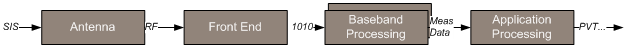
\includegraphics[width=0.7\textwidth]{modelPOR}
	\caption{Funkcionalni model programski određenog radio prijamnika za satelitsku navigaciju}
	\label{Fig:modelPOR}	
\end{figure}

Za područje satelitske navigacije, domena visokih frekvencija izdvojit će i digitalizirati signale koji prenose PRN kodne sekvence i navigacijsku poruku. Nizovi brojeva prosljeđuju se u domenu osnovnog frekvencijskog područja koja identificira i izdvaja prenošene informacije. U satelitskom navigacijskom prijamniku, u ovoj se domeni postupakom unakrsne korelacije primljenih i lokalno generiranih PRN kodnih sekvenci određuju pseudoudaljnosti i izdvajaju elementi navigacijske poruke. U domeni aplikacijskog procesiranja, izlaz osnovnog frekvencijskog područja bit će obrađeni s ciljem spremanja informacija u korisniku razumljivom obliku (Slika \ref{Fig:modelPOR}).

\section{Pojam programski određenog radioprijemnika}
Tradicionalni prijamnik za satelitsku navigaciju je izveden sklopovski. Elektronički sklopovi posebne namjene obavljaju ciljane funkcije unutar segmenata prijamnika. Pri tome, konstrukcija i izvedba sklopova definira uspješnost primjene matematičkih modela u ispunjavanje traženih funkcionalnosti, odnosno postavljenih zahtjeva na kvalitetu procesiranja signala i informacija.

Elektronički sklopovi su po svojoj su prirodi nesavršeni i ograničeni. Jednom konstruirani i izvedeni elektronički sklopovi posebne namjene ne mogu se lako značajnije promijeniti. Pokaže li se potreba za proširivanjem ili prilagođavanjem novom statusu sustava kao cjeline,
potrebno je napuštanje izvedbe starog sustava i konstrukcija ili kupnja potpuno nove.
U slučaju satelitske navigacije, tradicionalni GPS prijamnik, u kojem je generiranje PRN satelitskih sekvenci izvedeno sklopovskim načinom, uvođenje novih satelita i modernizacija sustava izazivaju napuštanje starog i konstrukciju ili kupnju potpuno novog i kompatibilnog GPS prijamnika.

Dvadesete godine dvadesetog stoljeća uvode novi koncept radiokomunikacijske tehnologije.
Reducira se broj elektroničkih sklopova posebne namjene i uvode programske komponente za obradu signala i informacija. Time se omogućava lakše praćenje promjena sustava i izravnija primjena matematičkih modela u algoritamskom obliku na podglgama opće namjene, npr. osobna računala ili pametni telefoni.
Novi koncept se naziva programski određen radio (engl. Software-Defined Radio, SDR).
Lakoća prilagodbe promjenama, omogućila je SDR-u da ubrzo postane standard u radiokomunikacijskoj industriji.
Brojni uređaju od pametnih telefona do radijskih i televizijskih prijamnika su izvedeni u obliku SDR-a. Takva izvedba im omogućava postizanje bolje prilagodljivosti, proširivosti, iskorištenja energije i lakše komunikacije s drugim računalnim uređajuma. 

Programska izvedba prijamnika za satelitsku navigaciju zanimljiva je sa stajališta računarne
znanosti. Primjena algoritama za procesiranje signala i informacija podržava raspodjeljivanje
arhitekture sustava. Potpuno procesiranje više ne treba biti u potpunosti izvedeno na jednom uređaju
(npr. pametnom telefonu ili samostalnom GNSS prijamniku) pa se dijelovi postupka obrade prebacuju na druge uređaje. Svaki korišteni uređaj svoj dio obrade obavljaja kvalitetnije i točnije uz jednostavnije
korištenje izvora dodatnih informacija koje mogu pridonijeti poboljšanju točnosti procjene
položaja \cite{ref:46,ref:47}. Navedeni pristup omogućava korištenje računalnog okruženja u
oblaku što dopušta da se prijemniku ostavi samo obrada signala i informacija u frekvencijskoj
domeni. Izlaz obrade signala i informacija u frekvencijskoj domeni pohranjuje se u binarnom obliku
u \textit{RINEX} formatu.

\textit{RINEX}\label{sssec:rinex}
(engl. Receiver Independent Exchange Format) je općeprihvaćena definicija
sahranjivanja izlaza obrade (navigacijskih) satelitskih signala u frekvencijskoj domeni (neobrađeni podatci satelitske navigaciju).
Definiranje općeprihvaćenog načina sahranjivanja omogućava lako prebacivanje dijelova obrade 
na druge uređaje u svrhu poboljšanju točnosti procjene
položaja \cite{ref:46,ref:47}.
\textit{RINEX} se mijenja kroz vrijeme obuhvaćajući promjene GNS sustava. Trenutna verzija je
3.03 iz 2015 \cite{rinex:303}.

\section{Programski određen GPS prijemnik}
Programsko određen GPS prijemnik predstavlja vrstu programski određenog radioprijemnika posebne namjene,  procjene položaja satelitskim navigacijskim sustavima.

Posebnosti programski određenog radioprijemnika za potrebe
satelitske navigacije izražene su karakterističnim postupcima procesiranja signala i informacija u
domeni osnovnog frekvencijskog područja i domeni navigacijskog (aplikacijskog) procesiranja.
Karakteristični postupci su vezani za:
\begin{itemize}
	\item prihvat signala (engl. Acquisition), prepoznavanje PRN kodne sekvence pojedinačnog
	satelitskog signala,
	\item sljeđenje signala (engl. Tracking), vremensko usklađivanje s primljenim signalom, za
	potrebe kasnijeg određivanja pseudoudaljenosti,
	\item procjena vidljivosti satelita,
	\item procjena položaja, brzine i vremena.
\end{itemize}

%PREVESTI SLIKU
%NAĆI RAZUMLJIVIJU SLIKU
\begin{figure}[H]
	\centering
	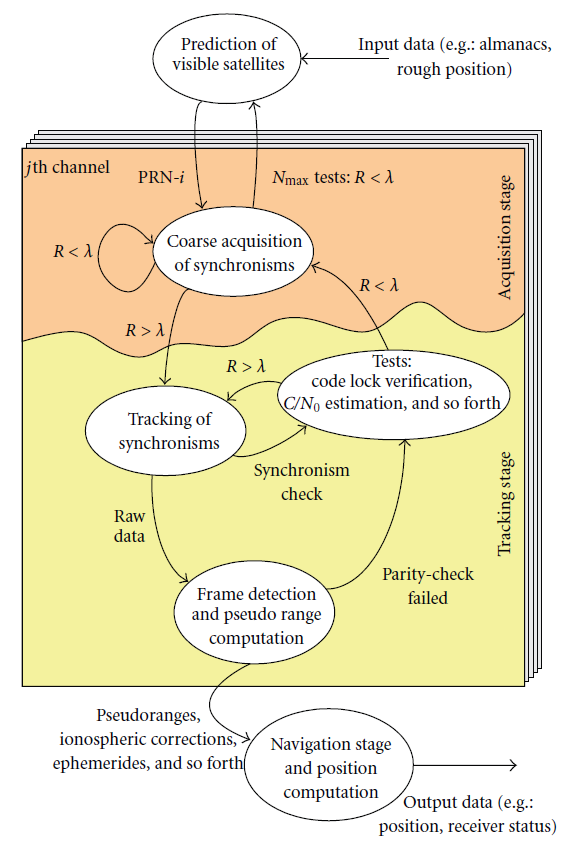
\includegraphics[width=0.7\textwidth]{prihvatSignala}
	\caption{Procesiranje signala u domeni osnovnog frekvencijskog područja}
	\label{Fig:prihvat}	
\end{figure}

Procesiranje signala u domeni osnovnog frekvencijskog područja (Slika \ref{Fig:prihvat}) obuhvaća prihvat
signala, sljeđenje signala, izdvajanje navigacijske poruke i određivanje pseudoudaljenosti. Obavlja se
na razini komunikacijskog kanala,tj. za svaki pojedinačni satelitski signal. U slučaju gubitka
vremenske usklađenosti s primljenim signalom, prijamnik će prijeći na prihvat signala, dok se ne
stvore uvjet za ponovni prijelaz u fazu slijeđenja. U slučaju potpunog gubitka signala, prijemnik ponovo započinje postupak prihvata.

Algoritmi obrade signala u domeni osnovnog frekvencijskog područja ovise o spremnosti procjene vidljivosti satelita koja se u navigacijskoj domeni zasniva na pojednostavljenom
opisu satelitskih putanja, efemeridama. Almanah o statusu satelita u "sazviježđu", kao i satelitske efemeride, se prenose navigacijskom porukom. Promjene almanaha obavljaju se na
dnevnoj bazi. Ukoliko prijamnik već poznaje dnevni almanah, je u stanju brže napraviti
prvu procjenu položaja, što se naziva topli start GPS (ili općenito GNSS) prijamnika.
Ukoliko su prijamniku poznati i dnevni almanah i efemeride, vrijeme do prve procjene položaja je još kraće (nekoliko desetaka sekundi) što nazivamo vrući start GNSS prijamnika. Ako
prijamnik nema ni dnevni alamanh ni sateliske efemeride, vrijeme do procjene položaja
može biti prilično dugo. Ono ovisi o načinu dobavljanja navigacijske poruke. Ako se poruka
prima sa satelita, vrijeme do prve procjene položaja je barem 12.5 min.Takvo stanje GNSS prijamnika se naziva hladan start GNSS prijamnika. Hladan start je moguće ubrzati alternativnom dostavom navigacijske poruke, npr. preko
telekomunikacijskih mreža. Naime, elementi telekomunikacijskih mreža su vremenski usklađeni pomoću satelitskih
navigacijskih prijamnika pa čvorovi mreže već poznaju navigacijsku poruku i mogu je prenijeti
korisničkoj opremi (GNSS prijemniku). Način rada u kojem
korisnički prijamnik ne prima sve potrebne podatke za određivanje položaja putem satelita nazivamo potpomognutom satelitskom navigacijom (engl. Augmented GNSS, A-GNSS).

Algoritam procesiranja informacija u domeni navigacijske primjene (Poglavlje \ref{sec:algoritam}) koristi informacije iz
navigacijske poruke (satelitske efemeride, alamanah i parametre modela ispravaka pogrešaka) te
izmjerene pseudoudaljenosti kako bi se procijenio položaj (i/ili brzinu) prijemnika i ispravio
pogrešku korisničkog sata. Modelima ispravaka ispravljaju se poznate sustavne pogreške
položaja satelita, ionosferskog i troposferskog kašnjenja te pogreške korisničkog sata uključene u
izmjerene vrijednosti pseudoudaljenosti, čime se omogućuje točnija procjena
položaja (i/ili brzine i vremena). Slučajne pogreške ostaju nepokrivene pa procjena položaja nije
apsolutno točna. Naime, postupak procjene položaja omogućuje zadovoljavajuću procjenu pogreške
određivanja položaja. Ona se može predstaviti korisniku, zajedno s rezultatima procjene položaja (i/ili brzine i vremena).

\section{Praktična izvedba korisničkog GPS prijamnika}
U okvirima diplomskog rada izvaden je korisnički $GPS$ prijemnik.
Izvedeni radioprijemnik je moguće koristiti za obradu satelitskih signala i informacija u domeni osnovnog frekvencijskog područja i domeni navigacijske primjene. Obrada signala u domeni osnovnog frekvencijskog područja se izvodi korištenjem programske knjižnice otvorenog koda \textit{GNSS SDRLIB}
\cite{ref:48}. Obrada informacija u domeni navigacijske primjene je moguće izvesti korištenjem programskog paketa otvorenog koda \textit{RTKNAV} iz programske knjižnice \textit{RTKLIB}\cite{ref:36}.

\begin{figure}[H]
	\centering
	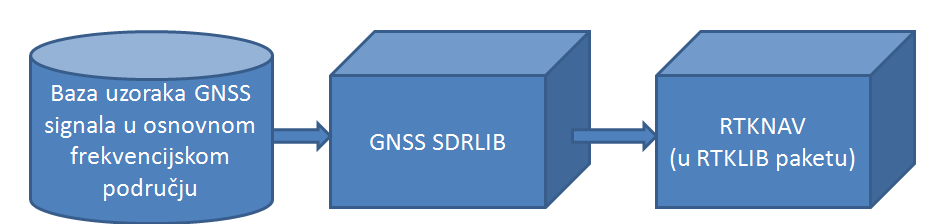
\includegraphics[width=0.7\textwidth]{rtkGNSS}
	\caption{Shema GNSS radioprijemnika}
	\label{Fig:radioprijemnik}	
\end{figure}
Spomenute knižnice povezane su klijentsko-poslužiteljskom arhitekturom.
\vspace{0.5cm}
Programska knjižnica \textit{GNSS SDRLIB} (Slika \ref{Fig:sdrlib}) omogućava korištenje kompozitnih
GPS signala (Slika \ref{Fig:GPSSignal}) u domeni osnovnog  frekvencijskog područja dostavljenih strujenjem
ili arhivkom datotekom.
Omogućuje izbor pojedinačnog GNSS sustava i pojedinačnih satelita pa tako i odabranog $GPS$ sustava.
Također, omogućava pristup strujanim podatcima potpomognutog GNSS-a,  dostavljanim putem internetske veze od trećih strana (dobavljača ispravaka).
\begin{figure}[H]
	\centering
	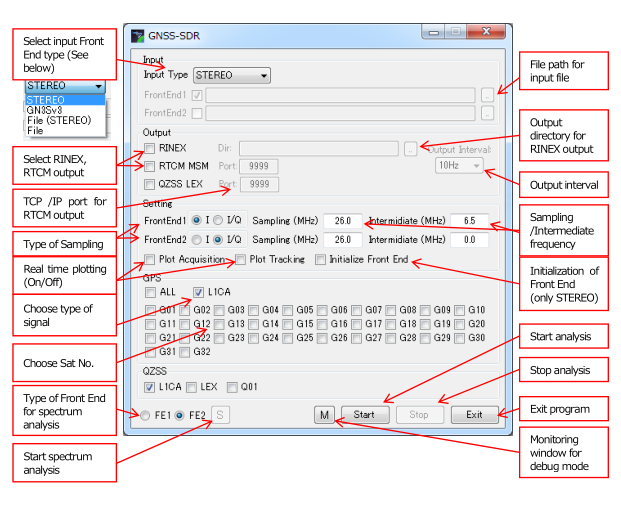
\includegraphics[width=0.8\textwidth]{sdrlib}
	\caption{Grafičko korisničko sučelje programskog paketa GNSS-SDRLIB}
	\label{Fig:sdrlib}	
\end{figure}
%
Programski paket \textit{RTKNAVI} je dio programske knjižnice otvorenog koda \textit{RTKLIB} \cite{ref:36, ref:5}.
Koristi se za procjenu položaja (i/ili brzine i vremena) zasnovanom na podatcima
(pseudoudaljenosti i sadržaja navigacijske poruke) koji čine izlaz domene za obradu signala u osnovnom
frekvencijskom području. Preko grafičkog korisničkog sučelja (Slike \ref{Fig:rtkNav} i \ref{Fig:guirtkNav}) omogućuje
praćenje statusa procesa: toka podataka iz GNSS SDRLIB aplikacije prema RTKNAV aplikaciji,
grafičkog predstavljanja jakosti prihvaćenih i sljeđenih satelitskih signala te procjenu navigacijskih
parametara (tri komponente položaja: geografska širina, geografska dužina i nadmorska visina,
brzina i točno vrijeme) temeljem mjerenih vrijednosti pseudoudaljenosti korištenih
satelita te uz korištenje temeljnog postupka procjene položaja i točnog
vremena (Slika \ref{Fig:rtkNavKo}). 
Korišteni algoritmi procesiranja informacija i procjene
položaja opisani su u dokumentraciji programske knjižnice RTKLIB \cite{ref:36}.
\begin{figure}[H]
	\centering
	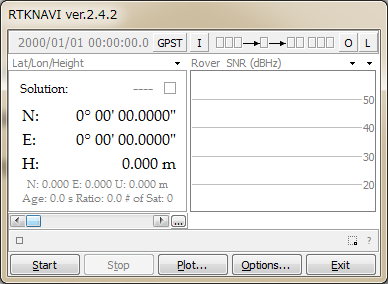
\includegraphics[width=0.6\textwidth]{rtkNav}
	\caption{Grafičkko korisničko sučelje programskog paketa RTKNAV}
	\label{Fig:rtkNav}	
\end{figure}
\begin{figure}[H]
	\centering
	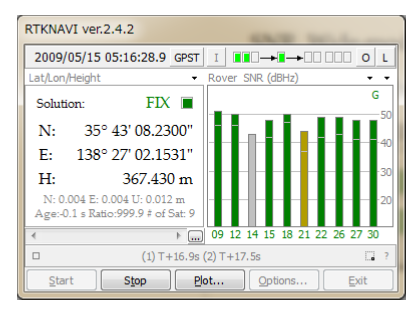
\includegraphics[width=0.6\textwidth]{guirtkNav}
	\caption{GUI RTKNAV aplikacije u radu (zastavica FIX označava ispravnu procjenu položaja)}
	\label{Fig:guirtkNav}	
\end{figure}
\begin{figure}[H]
	\centering
	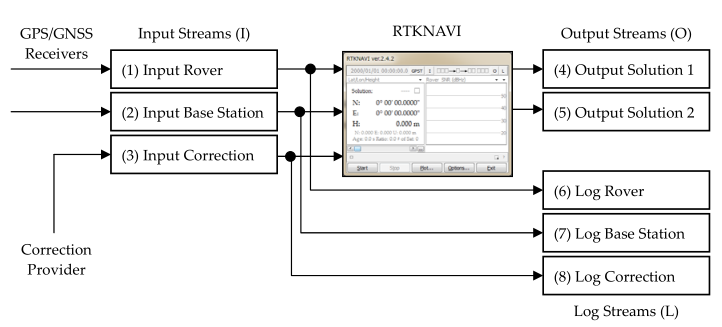
\includegraphics[width=0.8\textwidth]{rtkNavKo}
	\caption{Korištenje aplikacije RTKNAV, s ulaznim i izlaznim informacijama}
	\label{Fig:rtkNavKo}	
\end{figure}

Korišteni uzorci GPS signala u domeni osnovnog frekvencijskog područja su pribavljeni eksperimantalno izvedenim GPS prijemnik u stvarnim uvjetima.
Nad njima je obavljena obrada signala u frekvencijskoj domeni i potrebni podatci za ulaz u 
algoritme procjene položaja u domeni navigacijske primjene su spremljeni u tekstualnom obliku (koordinate satelita i pripadne pseudoudaljenosti).

\chapter{Praktična izvedba procjene položaja u domeni navigacijske primjene}\label{sec:izvedba}
Algoritmi procjene položaja u domeni navigacijske primjene su opisani u dokumentaciji programske knjižnice RTKLIB \cite{ref:36}.
Osnovni algoritam čini algoritam najmanjih kvadrata predstavljen algoritmom \ref{code:iterLSM} sa \pageref{code:iterLSM} stranice ovoga rada. Poboljšanje osnovnog algoritma ostvareno je uvođenjem odgovarajućih težina, odnosno upotrebom algoritma \ref{code:iterLSMW} sa stranice \pageref{code:iterLSMW}.

Za dobivene psudoudaljenosti i 
položaj satelita u \textit{ECEF XYZ} koordinatnom sustavu algoritmi izračunavaju položaj
prijemnika i pogrešku sata prijemnika. Izvedba algoritama, ostvarena je korištenjem programskog jezika $R$ \cite{ref:24} i R-sučelja \textit{RStudio} na GNU/Linux operativnom sustavu.
\section{Programski jezik R}
$R$ je programski jezik za statističku i drugu matematičku obradbu putem računala i ima snažnu grafičku potporu.
Između ostalog, podržava postupke zasnovane na linearnoj algebri, analizi i prognozi ponašanja vremenskih nizova i grafičkom predočavanju \cite{ref:34,ref:22}.
Pogodan je za izvedbu statističke analize, modeliranje i simulacije.
 
 \textit{R} je dostupan za većinu korištenih platformi (Microsoft Windows, Linux, Mac OS X), a instalacija je poprilično jednostavna.
 Potrebno je samo preuzeti potrebne datoteke s web-stranice \cite{Rsite} i u skladu s njima instalirati program.
 Instalirani program nudi R-sučelje (R-GUI) u kojemu se preko naredbene linije zadaju naredbe i pokreću skripte, a dobivaju numerički i grafički rezultati.
 Postoji i više neslužbenih R-sučelja. Jedan od poznatijih je \textit{R-Studio} \cite{RStudio}.
 Ovdje se komunikacija opet ostvaruje preko naredbi u konzoli, ali je RStudio opremljen znantno bogatijom grafičkom okolinom (radni prostor, povijest, instalacija paketa, pomoć i sl.).
Postoji i mogućnost integracije $R$ interpretera u odabrani tekst-editor ili poziva R-funkcija iz drugih programskih jezika (Python, Ruby, SAGE).
\\

 U izradi ovoga teksta korišten je programski jezik R sa standardnim i dodatnim (\textit{MASS}, \textit{matlib}, \textit{limSolve} i \textit{matrixcalc}) programskim knjižnicama \cite{ref:4,ref:6,ref:8}.

\section{Osnovni pristup}
Sustav koji opisuje problem određivanja položaja je nelineraran pa
ga možemo prvo \textbf{linearizirati}, a tek zatim primjeniti metodu najmanjih kvadrata \cite{googleSchoolar1}.
Općenito, rješenja lineariziranog i nelineariziranog sustava nisu u potpunosti jednaka \cite{singer07}, ali su u ovom slučaju dovoljno bliska. Naime, jednadžbe sustava su skoro linearne.%slide 16

\subsection{Prvi način linearizacije jednadžbi sustava}
Prvi način linearizacije jednadžbi sustava dobivamo promatrajući sustav \ref{eq:1}:
\begin{align}\label{eq:1partial}
d_1 = \sqrt{(x-x_1)^{2}+(y-y_1)^{2}+(z-z_1)^{2}} + c\cdot d_T \notag \\
d_2 = \sqrt{(x-x_2)^{2}+(y-y_2)^{2}+(z-z_2)^{2}} + c\cdot d_T  \\
d_3 = \sqrt{(x-x_3)^{2}+(y-y_3)^{2}+(z-z_3)^{2}} + c\cdot d_T \notag \\
d_4 = \sqrt{(x-x_4)^{2}+(y-y_4)^{2}+(z-z_4)^{2}} + c\cdot d_T \notag
\end{align}
u $\mathbf{x} = (x,y,z,d_T)$.\\
Označimo s $f_i(\mathbf{x}) = \sqrt{(x-x_1)^{2}+(y-y_1)^{2}+(z-z_1)^{2}} + c\cdot d_T$.\\
Linearizacijom jednadžbi sustava na isti način kao $\mathbf{p}(\mathbf{x})$ sa stranice \pageref{stranica:NGLin} (za Gauss-Newtonovu metodu), dobivamo:
\begin{align*}
f_i(\mathbf{x} + \Delta\mathbf{x}) = f_i(\mathbf{x}) + \frac{\partial f}{\partial x}\Delta x + \frac{\partial f}{\partial y}\Delta y + \frac{\partial f}{\partial z}\Delta z + \frac{\partial f}{\partial d_T}\Delta d_T 
\end{align*}
Koristeći iterativnu metodu, $\mathbf{x}_{k+1} = \mathbf{x}_k+\Delta\mathbf{x}_k$.
Budući da se $(d_1,d_2,d_3,d_4)$ ne mijenjaju kroz iteracije, dobivamo izraz:
$$
d_i = f_i(\mathbf{x}_{k+1}) = f_i(\mathbf{x}_{k} + \Delta\mathbf{x}_{k}) = f_i(\mathbf{x}_{k}) + \frac{\partial f}{\partial x}\Delta x_k + \frac{\partial f}{\partial y}\Delta y_k + \frac{\partial f}{\partial z}\Delta z_k + \frac{\partial f}{\partial d_T}\Delta (d_T)_k 
$$odnosno
\begin{align*}
d_i - \sqrt{(x_k-x_i)^{2}+(y_k-y_i)^{2}+(z_k-z_i)^{2}} - c\cdot (d_T)_k & = \\
\frac{\partial f}{\partial x}\Delta x_k + \frac{\partial f}{\partial y}\Delta y_k + \frac{\partial f}{\partial z}\Delta z_k + \frac{\partial f}{\partial d_T}\Delta (d_T)_k &= 
\begin{bmatrix}
\frac{\partial f_i}{\partial x} &
\frac{\partial f_i}{\partial y} &
\frac{\partial f_i}{\partial z} &
\frac{\partial f_i}{\partial d_T}
\end{bmatrix}
\begin{bmatrix}
\Delta x \\
\Delta y \\
\Delta z \\
\Delta d_T
\end{bmatrix} \\ 
\end{align*}
Uz 
\begin{align}
\mathbf{A} & := \begin{bmatrix}
\frac{\partial f_1}{\partial x} &
\frac{\partial f_1}{\partial y} &
\frac{\partial f_1}{\partial z} &
\frac{\partial f_1}{\partial d_T} \\
\frac{\partial f_2}{\partial x} &
\frac{\partial f_2}{\partial y} &
\frac{\partial f_2}{\partial z} &
\frac{\partial f_2}{\partial d_T} \\
\frac{\partial f_3}{\partial x} &
\frac{\partial f_3}{\partial y} &
\frac{\partial f_3}{\partial z} &
\frac{\partial f_3}{\partial d_T} \\
\frac{\partial f_4}{\partial x} &
\frac{\partial f_4}{\partial y} &
\frac{\partial f_4}{\partial z} &
\frac{\partial f_4}{\partial d_T}
\end{bmatrix} \\
& = \begin{bmatrix}
\frac{(x-x_1)}{\sqrt{(x-x_1)^{2}+(y-y_1)^{2}+(z-z_1)^{2}}} & \frac{(y-y_1)}{\sqrt{(x-x_1)^{2}+(y-y_1)^{2}+(z-z_1)^{2}}} & \frac{(z-z_1)}{\sqrt{(x-x_1)^{2}+(y-y_1)^{2}+(z-z_1)^{2}}} & c \\
\frac{(x-x_2)}{\sqrt{(x-x_2)^{2}+(y-y_2)^{2}+(z-z_2)^{2}}} & \frac{(y-y_2)}{\sqrt{(x-x_2)^{2}+(y-y_2)^{2}+(z-z_2)^{2}}} & \frac{(z-z_2)}{\sqrt{(x-x_2)^{2}+(y-y_2)^{2}+(z-z_2)^{2}}} & c \\
\frac{(x-x_3)}{\sqrt{(x-x_3)^{2}+(y-y_3)^{2}+(z-z_3)^{2}}} & \frac{(y-y_3)}{\sqrt{(x-x_3)^{2}+(y-y_3)^{2}+(z-z_3)^{2}}} & \frac{(z-z_3)}{\sqrt{(x-x_3)^{2}+(y-y_3)^{2}+(z-z_3)^{2}}} & c \\
\frac{(x-x_4)}{\sqrt{(x-x_4)^{2}+(y-y_4)^{2}+(z-z_4)^{2}}} & \frac{(y-y_4)}{\sqrt{(x-x_4)^{2}+(y-y_4)^{2}+(z-z_4)^{2}}} & \frac{(z-z_4)}{\sqrt{(x-x_4)^{2}+(y-y_4)^{2}+(z-z_4)^{2}}} & c \\
\end{bmatrix}\\
\mathbf{x} & :=  \begin{bmatrix}
\Delta x \\
\Delta y \\
\Delta z \\
\Delta d_T
\end{bmatrix}\\
\mathbf{b} & := \begin{bmatrix}
d_1 - \sqrt{(x_k-x_1)^{2}+(y_k-y_1)^{2}+(z_k-z_1)^{2}} - c\cdot (d_T)_k \\
d_2 - \sqrt{(x_k-x_2)^{2}+(y_k-y_2)^{2}+(z_k-z_2)^{2}} - c\cdot (d_T)_k \\
d_3 - \sqrt{(x_k-x_3)^{2}+(y_k-y_3)^{2}+(z_k-z_3)^{2}} - c\cdot (d_T)_k \\
d_4 - \sqrt{(x_k-x_4)^{2}+(y_k-y_4)^{2}+(z_k-z_4)^{2}} - c\cdot (d_T)_k
\end{bmatrix}
\end{align}%ISTO DEFF NA STR 41 http://www2.imm.dtu.dk/pubdb/views/edoc_download.php/2804/pdf/imm2804.pdf
dobivamo sustav:
\begin{align}\label{eq:sustav}
\mathbf{A}\mathbf{x} = \mathbf{b}
\end{align}
koji rješavamo metodom iterativnih najmanjih kvadrata.\label{stranica:nastavakLS}
Budući da zbog pogreške u mjerenjima ili linearizacije sustav \ref{eq:sustav} nema uvijek rješenje, tj. 
$\mathbf{A}\mathbf{x} - \mathbf{b} \not = 0, \forall \mathbf{x} \in \R^m$,
ideja je ne tražiti rješenje sustava, već $\mathbf{x}$ koji minimizira izraz $\|\mathbf{A}\mathbf{x} - \mathbf{b}\|_2$.
Prema sljedećem teoremu, dovoljno je promatrati sustav
$$ A^TA\mathbf{x} = A^Tb $$.

\begin{thm}
	Skup svih rješenja problema $\min_\mathbf{x}\| \mathbf{A}\mathbf{x} - \mathbf{b} \|_2$ označimo s
	$$ S= \{\mathbf{x} \in \R^\mathit{m} | \| \mathbf{A}\mathbf{x} - \mathbf{b} \|_2 \textit{ je minimalna} \} $$
	Tada je $\mathbf{x}  \in S$, tj. $\mathbf{x}$ je rješenje problema najmanjih kvadrata, ako i samo ako vrijedi sljedeća relacija ortogonalnosti 
	$$A^T(A\mathbf{x}-\mathbf{b}) = 0,$$
	\\ koju obično nazivamo \textit{sustav normalnih jednadžbi} i pišemo u obliku 
	$$ A^TA\mathbf{x} = A^Tb $$.
\end{thm}
\begin{proof}
Rješavanje problema $\mathbf{A}\mathbf{x} = \mathbf{b}$, gdje $\mathbf{x}$ parametar koji je potrebno odrediti, se svodi na prikaz vektora $\mathbf{b}$ u bazi koju čine stupci matrice $\mathbf{A}$. Ukoliko $\mathbf{b}$ nije iz prostora razapetog stupcima matrice $\mathbf{A}$, $L_A$,
tada je potrebno pronaći vektor $\mathbf{\hat{b}} \in L_A$ i
najbliži vektoru $\mathbf{b}$ među svim vektorima iz $L_A$.
Po definiciji, $\mathbf{\hat{b}}$ je projekcija $\mathbf{b}$ na $L_A$ dan formulom:
\begin{align*}
\mathbf{\hat{b}} := \mathbf{A(A^TA)^{-1}A^T}\mathbf{b}
\end{align*}
\begin{figure}[H]
	\centering
	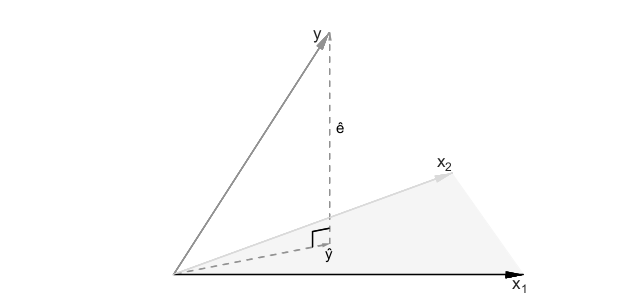
\includegraphics[width=0.8\textwidth]{linProjection}
	\caption{Projekcija vektora $\mathbf{y}$ u prostor razapet vektorima $x_1$ i $x_2$ \cite{svd_str15} }
	\label{Fig:projection}	
\end{figure}

$\mathbf{A(A^TA)^{-1}A^T}$ nazivamo projektor na prostor razapet stupcima matrice $\mathbf{A}$ i obično označavamo s $\mathbf{H}$.\\
Vrijedi da je $\mathbf{\hat{x}}$ rješenje problema najmanjih kvadrata ako i samo ako
vrijedi $\mathbf{A}\mathbf{\hat{x}} = \mathbf{\hat{b}}$, tj.
$\mathbf{\hat{x}}:= \mathbf{(A^TA)^{-1}A^T}\mathbf{b}$\label{eq:lin1Xeq}. Zaključujemo kako je $\mathbf{\hat{x}}$ rješenje problema najmanjih kvadrata ako i samo ako je $\mathbf{\hat{x}}$ \textbf{rješenje problema normalnih jednadžbi}
\begin{align}\label{eq:sustavProj}
A^TA\mathbf{x} = A^Tb.
\end{align}
\end{proof}

Detaljniji dokaz teorema može se pronaći u \cite{singer07}, stranica 46.\\

Zanimljivo je da poznavajući
 jedno rješenje sustava \ref{eq:sustavProj}, relativno je lagano pronaći i sva ostala.\\
Naime, uz $\mathbf{A}\mathbf{x} - \mathbf{b} = r$ i proizvoljan $\hat{\mathbf{x}} \in \R^m$ za koji vrijedi
\begin{align}
\hat{r}  &=  \mathbf{A}\mathbf{\hat{x}} - \mathbf{b} \notag \\
&= A\mathbf{\hat{x}} + r - A\mathbf{x}\notag \\
&= r + A(\mathbf{\hat{x}} - \mathbf{x}) \notag
\end{align}
imamo da je $\mathbf{\hat{x}} \in S$ ako i samo ako $\hat{r} = r$, tj.  $ A(\mathbf{\hat{x}} - \mathbf{x}) = 0$ i $\mathbf{\hat{x}} - \mathbf{x} \in \mathcal{N}(A)$.\\
Također, ukoliko vrijedi nešto od sljedećega:%
\begin{itemize}
	\item $A$ ima puni stupčani rang,
	\item stupci matrice $A$ su linearno nezavisni,
	\item $A^TA$ je pozitivno definitna,
\end{itemize}
$\mathcal{N}(A)$ je trivijalan i rješenje sustava je jedinstveno. 
\vspace{0.2cm}
\\Vrijedi i sljedeće:%
\begin{enumerate}
	\item Općenito, matrica $A^TA$ je simetrična i pozitivno semidefinitna jer za svaki
	$\mathbf{x} \in \R^m$ vrijedi
	$$  \mathbf{x}^TA^TA\mathbf{x} = (A\mathbf{x})^T(A\mathbf{x}) = \|A\mathbf{x}\|_2^2 \geq 0. $$
	\item Sustav normalnih jednadžbi uvijek ima rješenje i to jedinstveno.
\end{enumerate}
\vspace{1cm}
Nakon formalizacije problema, potreban je jednostavan način za izračunavanje rješenja sustava \ref{eq:sustavProj}.
Jasno je da se matrica $A^TA$ ne invertira, nego se rješava sustav \ref{eq:sustavProj}.
Sustav možemo rješiti tako što koristimo faktorizaciju Choleskoga matrice $A^TA$.
Tako pronađeno rješenje nije naročito točno\cite{singer07}, stranica 60.

\subsection{Drugi način linearizacije jednadžbi sustava}
Ponovno se promatra isti sustav jednadžbi \ref{eq:1}, ali se 
metoda iterativnih najmanjih kvadrata ne primjenjuje direktno na početni sustav, već na njegovu modifikaciju, modifikaciju sustava \ref{eq:new}.
Modificirani sustav je u mogućnosti dati isto dobro rješenje uz uvijet $cd_T < d_i, \forall i \in \{1,2,3,4\}$. \\

Prebacujući član $d=d_T \cdot c$ na lijevu stranu i kvadrirajući obje strane
jednadžbi sustava \ref{eq:new} dobivamo modificirani sustav jednadžbi:
\begin{align}\label{eq:newIzvedba}
(d_1-d)^2 = (x-x_1)^{2}+(y-y_1)^{2}+(z-z_1)^{2} + p_1(\textbf{x})\notag \\
(d_2-d)^2 = (x-x_2)^{2}+(y-y_2)^{2}+(z-z_2)^{2} + p_2(\textbf{x})\\
(d_3-d)^2 = (x-x_3)^{2}+(y-y_3)^{2}+(z-z_3)^{2} + p_3(\textbf{x})\notag \\
(d_4-d)^2 = (x-x_4)^{2}+(y-y_4)^{2}+(z-z_4)^{2} + p_4(\textbf{x})\notag
\end{align}
gdje je 
\begin{align*}
p_i(\textbf{x}) & = 2\sqrt{(x-x_i)^{2}+(y-y_i)^{2}+(z-z_i)^{2}}v_i + v_i^2.
\end{align*} i
\begin{align*}
p_i(\textbf{x}) & = (d_i-d)^2 - (x_i-x)^{2} - (y_i-y)^{2} - (z_i-z)^{2}.
\end{align*}
Označimo 
\begin{align*} \mathbf{\tilde{p}}(\mathbf{x}) := (p_1(\textbf{x}),p_2(\textbf{x}),p_3(\textbf{x}),p_4(\textbf{x}))^T
\end{align*}
pa minimizacijski problem \ref{eq:minimization} prelazi u
\begin{align}\label{eq:minimisation3}
\hat{\mathbf{x}} = \text{arg min}_\mathbf{x} \mathbf{\tilde{p}}(\mathbf{x})^T\mathbf{\tilde{p}}(\mathbf{x}).
\end{align}
Analogno \ref{eq:minimisation2} prelazi u 
\begin{align}\label{eq:minimisation4}
\hat{\mathbf{x}} = \text{arg min}_\mathbf{x} \mathbf{\tilde{p}}(\mathbf{x})^T \Sigma ^{-1}\mathbf{\tilde{p}}(\mathbf{x}).
\end{align}
\vspace{0.5cm}
Nadalje, $$ \mathbf{\tilde{p}'}(\mathbf{x}) = (p_1'(\textbf{x}),p_2'(\textbf{x}),p_3'(\textbf{x}),p_4'(\textbf{x}))^T 
= \begin{bmatrix}
2(x_1-x) &  2(y_1-y) &  2(z_1-z) & - 2c(d_1-cd_T)\\
2(x_2-x) &  2(y_2-y) &  2(z_2-z) & - 2c(d_2-cd_T) \\
2(x_3-x) &  2(y_3-y) &  2(z_3-z) & - 2c(d_3-cd_T) \\
2(x_4-x) &  2(y_4-y) &  2(z_4-z) & - 2c(d_4-cd_T) 
\end{bmatrix}
$$
\\Označimo s 
\begin{align*}
& P := \begin{bmatrix}
(x_1-x) & (y_1-y) & (z_1-z) & (d_1-d) \\
(x_2-x) & (y_2-y) & (z_2-z) & (d_2-d) \\
(x_3-x) & (y_3-y) & (z_3-z) & (d_3-d) \\
(x_4-x) & (y_4-y) & (z_4-z) & (d_4-d) 
\end{bmatrix} \\
& \tilde{I} := diag(1,1,1,-c).
\end{align*}
$$ \mathbf{\tilde{P'}}:= 2 P\tilde{I} $$
Imamo $$
\Delta \mathbf{x_k} = -(2 \Sigma^{-\frac{1}{2}} P\tilde{I} )^{-1}(\Sigma^{-\frac{1}{2}}\mathbf{\tilde{p}}(\mathbf{x_k}))
\\= -\frac{1}{2}(\Sigma^{-\frac{1}{2}} P\tilde{I} )^{-1}(\Sigma^{-\frac{1}{2}}\mathbf{\tilde{p}}(\mathbf{x_k})).
$$
Uz oznake,  
\begin{align}
\mathbf{A} := \mathbf{\tilde{P'}} \notag\\
\mathbf{b} := - \mathbf{\tilde{p}}(\mathbf{x_k}) \notag \\
\end{align}
u svakoj iteraciji algoritama \ref{code:iterLSM}
$\Delta \mathbf{x_k}$ računamo rješavajući sustav
\begin{align}\label{eq:drugaFakt}
\mathbf{A} \mathbf{x} = \mathbf{b}
\end{align}
za $\mathbf{x}:= \Delta \mathbf{x_k}$.
\\
Analogno u algoritmu \ref{code:iterLSMW}.

\subsection{Numeričke metode koje potpomažu rješavanje dobivenog (lineariziranog) sustava}
\subsubsection{QR dekompozicija}
Budući da će korištena matrica $A$ imati puni stupčani rang, rješenje problema minimizacije možemo zapisati kao:
\begin{align}\label{eq:useQR}
\| \mathbf{A}\mathbf{x} - \mathbf{b} \|_2	
& = \| \mathbf{Q}^T(\mathbf{A}\mathbf{x} - \mathbf{b}) \|_2 \\
& = \| \mathbf{Q}^T \mathbf{A}\mathbf{x} - \mathbf{Q}^T \mathbf{b} \|_2	\notag
\end{align}
gdje je $\mathbf{Q}$ proizvoljna ortogonalna matrica.\\
$\mathbf{Q}$ može bit proizvoljna pa možemo odabrati $\mathbf{Q}$ takvu da je lagano računati $\mathbf{x}$.
Ukoliko se koristi $Q$ iz \textit{QR} dekompozicije matrice $\mathbf{A}$ imamo $\mathbf{A} = \mathbf{QR}$ i $\mathbf{Q}^T\mathbf{A} = \mathbf{R}$ i $\mathbf{R}$ je gornjetrokutasta matrica.
Dalje rješavamo sustav
\begin{align}\label{eq:sustavQR}
\mathbf{R}\mathbf{x} = \mathbf{Q}^T\mathbf{b}.
\end{align}
tj. tražimo  
\begin{align*}
\mathbf{x} & = \mathbf{R}^{-1}\mathbf{Q}^T\mathbf{b} \\
& = \mathbf{R}^{-1}\mathbf{R}^{-T}\mathbf{R}^{T}\mathbf{Q}^T\mathbf{b} \\
& = (\mathbf{R}^{T}\mathbf{R})^{-1}(\mathbf{QR})^{T}\mathbf{b} \\
& = (\mathbf{R}^{T} \mathbf{I} \mathbf{R})^{-1}(\mathbf{QR})^{T}\mathbf{b}  \\
& = (\mathbf{R}^{T} \mathbf{Q}^T\mathbf{Q} \mathbf{R})^{-1}(\mathbf{A})^{T}\mathbf{b} \\
& = (\mathbf{A}^{T}\mathbf{A})^{-1}(\mathbf{A})^{T}\mathbf{b}
\end{align*}
Gledajući gornju jednakost odozdo prema gore, rješenje sustava nominalnih jednadžbi je jednako rješenju trokutastog sustava \ref{eq:sustavQR}.\\
Koristeći \textit{QR} dekompoziciju nije potrebno posebno uvoditi sustav nominalnih jednadžbi nego je dovoljno riješiti početni sustav jednadžbi. Dakle, u oba slučaja rješenje postoji i jedinstveno je.
%Kada to ne bi bio slučaj, moglo bi se dogoditi da sustav nema rješenja. Naime, prije primjene metode najmanjih kvadrata za pronalazak rješenja, linearizira se početni sustav jednadžbi i uvode se pogreške.
Rješenje dobiveno koristeći \textit{QR} dekompoziciju se pokazuje znatno točnije od rješenja dobivenog
direktnim računom $\mathbf{\hat{x}}:= \mathbf{(A^TA)^{-1}A^T}\mathbf{b}$ sa stranice \pageref{eq:lin1Xeq}.\\
\textit{QR} faktorizacija je pogodna za korištenje prilikom direktnog izračuna 
inverza općente matrice \textbf{A}:
\begin{align}
\mathbf{A}^{-1} = \mathbf{R}^{-1}\mathbf{Q}^{-1} = \mathbf{R}^{-1}\mathbf{Q^T}.
\end{align}
Primjetimo kako je \textbf{R} gornjetrokutasta pa je njezin inverz lakše izračunati.

\subsubsection{SVD dekompozicija}
\begin{defn}[SVD dekompozicija matrice]
	Neka je \textbf{A} $\in \R^{m\times n}$ ili $\C^{m \times n}$, $SVD$ dekompozicija matrice je $\mathbf{A} = \mathbf{UDV}^*$, $\mathbf{U} \in \R^{m\times m}$ ili $\C^{m\times m}$ unitarna matrica, $\mathbf{V} \in \R^{n\times n}$ ili $\C^{n\times n}$ unitarna matrica i $\mathbf{D} \in \R^{m\times n}$ nenegativna dijagonalna matrica. \\
	Nadalje, stupci matrice \textbf{U} su svojstveni vektori matrice $\mathbf{MM}^*$, dok su stupci matrice \textbf{V} 
	svojstveni vektori matrice $\mathbf{M}^*\mathbf{M}$. Dijagonalni elementi matrice $\mathbf{D}$ su korijeni svojstvenih vrijednosti matrice $\mathbf{M}^*\mathbf{M}$ ili $\mathbf{MM}^*$.
\end{defn}%
Inverz matrice \textbf{A} moguće je računati i pomoću \textbf{SVD} dekompozicije:%
\begin{align}
\mathbf{A}^{-1} := \mathbf{V}^{-*}\mathbf{D}^{-1}\mathbf{U}^{-1} := \mathbf{V}\mathbf{D}^{-1}\mathbf{U}^*
\end{align}
gdje je inverz dijagonalne matrice i hermistski adjugiranu matricu proizvoljne matrice lagano izračunati.

\textit{SVD} dekompoziciju je moguće koristiti i prilikom rješavanja sustava linearnih jednadžbi.
Matrice \textbf{A} sustava linearnih sustava ovoga rada su uvijek realne pa 
za \textbf{U},\textbf{D} i \textbf{V} matrice \textbf{SVD} dekompozicije matrice \textbf{A}
vrijedi $\mathbf{U}^* = \mathbf{U}^T$, $\mathbf{D}^* = \mathbf{D}^T = \mathbf{D}$ i $\mathbf{V}^* = \mathbf{V}^T$ i \textbf{U} i \textbf{V} su ortogonalne matrice.
Dakle, za \textbf{Q} u izrazu \ref{eq:useQR} se može uzeti \textbf{U}. Dobiva se:
\begin{align}\label{eq:useSVD}
\| \mathbf{A}\mathbf{x} - \mathbf{b} \|_2	
& = \| \mathbf{U}^T(\mathbf{A}\mathbf{x} - \mathbf{b}) \|_2 \\
& = \| \mathbf{U}^T \mathbf{A}\mathbf{x} - \mathbf{U}^T \mathbf{b} \|_2	\notag \\
& = \| \mathbf{D} \mathbf{V}^T\mathbf{x} - \mathbf{U}^T \mathbf{b} \|_2 \notag
\end{align}
Dalje se onda rješava sustav nominalnih jednadžbi
\begin{align}
(\mathbf{D} \mathbf{V}^T)^T\mathbf{D} \mathbf{V}^T\mathbf{x} 
& = (\mathbf{D} \mathbf{V}^T)^T\mathbf{U}^T \mathbf{b} \notag \\
\end{align} i rješenje za \textbf{x} je jednako
\begin{align}
	\mathbf{x} = \mathbf{V}\mathbf{D}^{-1}\mathbf{U}^T \mathbf{b}.
\end{align}
\textit{SVD} dekompozicija je pogodna za rješavanje nezasićenog sustava jednadžbi.\\
Za rješavanja prezasićenog sustava jednadžbi, boljom se pokazuje \textit{QR} dekompozicija.
\label{page:boljaQRzaSustav}%OBJ ZASTO BOLJE QR an ne svd u rj sustava

\subsection{Izvedba}
\subsubsection{Prvi način linearizacije}
Rješava se sustav \ref{eq:sustavQR} iterativnim postupkom.\\
Programski kod izvedbe se nalazi u dodatku \ref{appendix:izvedba} ovoga rada.\\
Programska izvedba postupka procjene položaja satelitskim navigacijskim sustavom napravljena je u poopćenom obliku. Podržava se slučaj procjene položaja s brojem izmjerenih pseudo-udaljenosti većim ili jednakim 4.
U svakoj iteraciji algoritma, $\Delta \mathbf{x}_k$ je pronađen kao rješenje sustava\\
$\mathbf{A}\mathbf{x} = \mathbf{b}$ \ref{eq:sustav}\\
metodom najmanjih kvadrata koristeći \textbf{QR} dekompoziciju, tj. rješavajući sustav \ref{eq:sustavQR}.

\subsubsection{Drugi način linearizacije}
Rješava se sustav \ref{eq:drugaFakt} iterativnim postupkom.\\
Programski kod izvedbe se nalazi u dodatku \ref{appendix:izvedba} ovoga rada.\\
Programska izvedba postupka procjene položaja satelitskim navigacijskim sustavom napravljena je u poopćenom obliku. Podržava se slučaj procjene položaja s brojem izmjerenih pseudo-udaljenosti većim ili jednakim 4.
Svaka iteracija algoritma pronalazi $\Delta \mathbf{x}_k$ je pronađen kao rješenje sustava\\
$\mathbf{A}\mathbf{x} = \mathbf{b}$ \ref{eq:drugaFakt}\\
metodom najmanjih kvadrata koristeći \textbf{QR} dekompoziciju.

\subsection{Rasprava o kvaliteti procjene položaja}
Kvaliteta procjene položaja satelitskim navigacijskim sustavom razmotrena je sa sljedećih stajališta:
\begin{itemize}
	\item potrebnog računalnog vremena za postizanje stabilne procjene u okruženju R,
	\item brzine konvergencije iteracijskog postupka,
	\item točnosti procjene koordinata položaja.
\end{itemize}

\subsubsection{Prvi način linearizacije}
Prvom izvedbom osnovnog algoritma za procjenu položaja dobivamo sljedeće rezultate:
\begin{table}[H]
	\caption{Kvaliteta prve izvedbe osnovnog algoritma za procjenu položaja u domani navigacijske primjene}
	%\rowcolors{1}{}{lightgray}
	\begin{center}
		\begin{tabular}{|p{3cm}|p{4cm}}
			\hline
			\rowcolor{lightgray}NAZIV&   \\
			\rowcolor{lightgray}&   \\
			\multirow{-3}{1cm}{ \cellcolor{lightgray}PARAMETRA} & \multirow{-3}{2cm}{\cellcolor{lightgray}VRIJEDNOST} \\
			\hline
			\vspace{0.1cm}
			vrijeme izvršavanja & \vspace{0.1cm}  43.42 za $10^5$ iteracija\\
			\vspace{0.1cm}
			broj iteracija do konvergencije & \vspace{0.1cm} $> 100000$ \\
			\vspace{0.1cm}
			točnost procjene & \vspace{0.1cm} $10^5$ \\
			\hline
		\end{tabular}
	\end{center}
\end{table}

\begin{figure}[H]
	\begin{minipage}{0.48\textwidth}
		\centering
			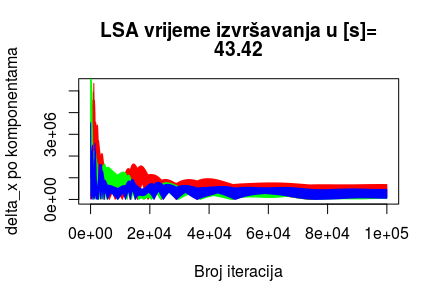
\includegraphics[width=1\textwidth]{1LSAdelta}
		\caption{Vrijednosti $\Delta x$ po komponentama kroz iteracija}
		\label{fig:1LSAdelta}
	\end{minipage}%	
	\hspace{1cm}
	\begin{minipage}{0.48\textwidth}
		
		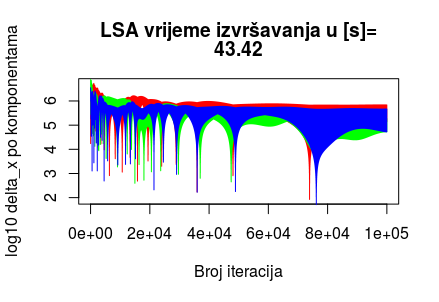
\includegraphics[width=1\textwidth]{1LSAdeltal10}
		\caption{Logaritam vrijednosti $\Delta x$ po komponentama kroz iteracije}
		\label{fig:1LSAdeltal10}
	\end{minipage}%
\end{figure}
Slike \ref{fig:1LSAdelta} i \ref{fig:1LSAdeltal10} pokazuju kako se izračunata pogreška ($\Delta \mathbf{x}$) procjene položaja nikada istovremeno ne spušta ispod $10^4$ za sve komponente procjene položaja. Algoritam nikada ne konvergira.
Još više, u svakoj iteraciji je izračunata pogreška veća od $10^4$ za barem dvije komponente.\\
Ukoliko smanjimo zahtjeve konvergencije algoritma na samo jednu komponentu ispod $10^2$ ili $10^3$,
metoda konvergira u 2000, odnosno 2400 iteracija. 
\begin{figure}[H]
	\begin{minipage}{0.48\textwidth}
		\centering
		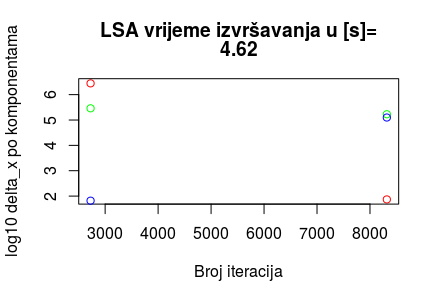
\includegraphics[width=1\textwidth]{1less100delta}
		\caption{Logaritam vrijednosti komponenata $\Delta \mathbf{x}$ kroz iteracije}
		\label{fig:1less100delta}
	\end{minipage}%	
	\hspace{1cm}
	\begin{minipage}{0.48\textwidth}
		\centering
		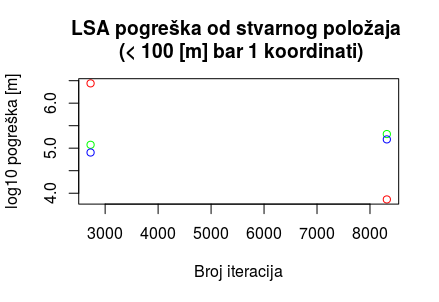
\includegraphics[width=1\textwidth]{1less100real}
		\caption{Logaritam pogreške određivanja položaja}
		\label{fig:1less100real}
	\end{minipage}%
\end{figure}
Slike \ref{fig:1less100delta} i \ref{fig:1less100real} prikazuju odnos izračunate pogreške u procjeni koordinata i stvarne pogreške u iteracijama u kojima je barem jedna komponenta $\Delta \mathbf{x}$
manja od 100.

\begin{figure}[H]
	\begin{minipage}{0.48\textwidth}
		\centering
		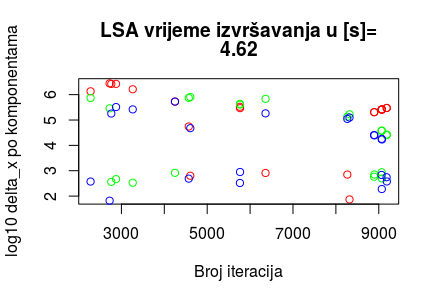
\includegraphics[width=1\textwidth]{1less1000delta}
		\caption{Logaritam vrijednosti komponenata $\Delta \mathbf{x}$ kroz iteracije }
		\label{fig:1less1000delta}
	\end{minipage}%	
	\hspace{1cm}
	\begin{minipage}{0.48\textwidth}
		\centering
		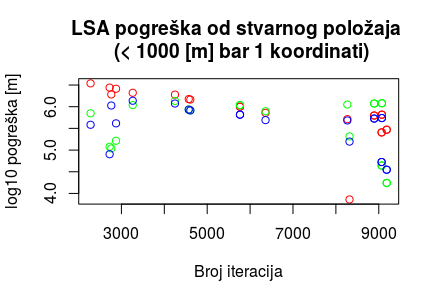
\includegraphics[width=1\textwidth]{1less1000real}
		\caption{Logaritam pogreške određivanja položaja}
		\label{fig:1less1000real}
	\end{minipage}%
\end{figure}
Slike \ref{fig:1less1000delta} i \ref{fig:1less1000real} prikazuju odnos izračunate pogreške u procjeni koordinata i stvarne pogreške u iteracijama u kojima je barem jedna komponenta $\Delta \mathbf{x}$
manja od 1000.

Vidljivo je da čak i u tim iteracijama
prava pogreška određivanja položaja ne silazi ispod $10^3$.
%ZELIMO POBOLJŠANJE

\subsubsection{Drugi način linearizacije}
Drugi naćin linearizacije daje drugu izvedbu osnovnog algoritma za procjenu položaja.
Promatrajući njegovu kvalitetu dobivamo sljedeće rezultate:
\begin{table}[H]
	\caption{Kvaliteta prve izvedbe osnovnog algoritma za procjenu položaja u domani navigacijske primjene}
	%\rowcolors{1}{}{lightgray}
	\begin{center}
		\begin{tabular}{|p{3cm}|p{4cm}}
			\hline
			\rowcolor{lightgray}NAZIV&   \\
			\rowcolor{lightgray}&   \\
			\multirow{-3}{1cm}{ \cellcolor{lightgray}PARAMETRA} & \multirow{-3}{2cm}{\cellcolor{lightgray}VRIJEDNOST} \\
			\hline
			\vspace{0.1cm}
			vrijeme izvršavanja & \vspace{0.1cm}  0.01\\
			\vspace{0.1cm}
			broj iteracija do konvergencije & \vspace{0.1cm} $> 6$ \\
			\vspace{0.1cm}
			točnost procjene & \vspace{0.1cm} $10^6$ \\
			\hline
		\end{tabular}
	\end{center}
\end{table}

\begin{figure}[H]
	\begin{minipage}{0.48\textwidth}
		\centering
		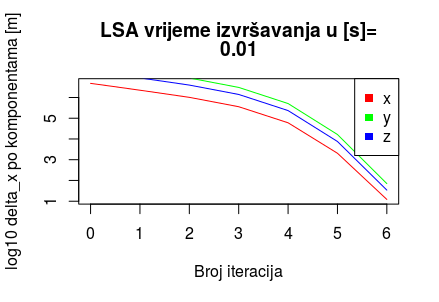
\includegraphics[width=1\textwidth]{2LSAdeltal10}
		\caption{Logaritam vrijednosti $\Delta x$ po komponentama kroz iteracije}
		\label{fig:2LSAdeltal10}
	\end{minipage}%	
	\hspace{1cm}
	\begin{minipage}{0.48\textwidth}
		
		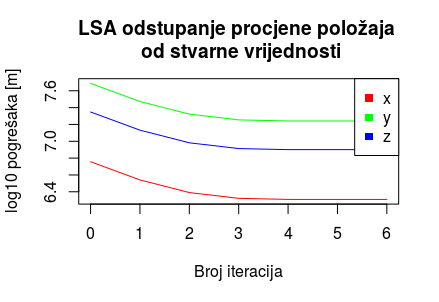
\includegraphics[width=1\textwidth]{2LSAreall10}
		\caption{Logaritam vrijednosti odstupanja od pravog položaja po komponentama kroz iteracije}
		\label{fig:2LSAreall10}
	\end{minipage}%
\end{figure}

Razmatrajući slike \ref{fig:2LSAdeltal10} i \ref{fig:2LSAreall10} vidljivo je kako druga izvedba
algoritma \ref{code:iterLSM} dovodi do konvergencije, ali ka krivom rješenju.\\
Dobivena procjena položaja ima odstupanje $10^6$.

%KAKVOĆA PREKO RMSE = σ̂^2 = hat(e)^T hat(e)/(N − p) p je broj nepoznatih varijabli 

\section{Poboljšan pristup: uvođenje težina (WLSM)}\label{sec:algTezine}%dipl4.R
Rezultati pokazuju kako do prezentirane metode ne mogu odrediti položaj ili određuju položaj prijemnika van okvira dopuštene točnosti.
Uzrok pronalazimo u pogreški mjerenja s utjecajem u ionosferi.\\
Iako pretpostavljamo da su pseudo-udaljenosti u potpunosti ispravljene, utjecaj ionosfere nije moguće u potpunosti reducirati jer koristimo samo jedan signal.
Naime, utjecaj ionosfere najbolje se otklanja korištenjem dva signala različitih frekvencija (s izvorom u istom satelitu). 
Literatura \cite{ref:4}, \cite{ref:9}, \cite{ref:10}, \cite{ref:38} i
\cite{ref:34} navodi kako je ionosfera jedna od najznačajnijih uzroka pogreške
procjene položaja.
Što je dulji put signala kroz ionosferu, to je utjecaj iononosfere veći i jednadžba pridružena tom signalu
je manje točna. Ukoliko je poznato da su neke jednadžbe sustav manje, a druge više točne, problem najmanih kvadrata
(stranica \pageref{code:iterLSM}) prelazi u problem težinskih najmanih kvadrata (stranica \pageref{code:iterLSMW}).
Svakoj jednadžbi pridjeljuje se koeficijent proporcionalan njezinoj točnosti.
Koeficijenti se modeliraju preko elevacijskog kuta satelita koji signal odašilje.
Veći elevacijski kut znači da će satelitski signal dulje putovati kroz ionosferu pa će pogreška
zbog ionosferskog kašnjenja biti veća (slika \ref{fig:elev}).
Uvažavajući navedeno i uz konzultaciju s literaturom \cite{ref:13}, \cite{ref:34},
\cite{ref:45} i \cite{ref:25} koristi se težinski koeficijent vezan za kut elevacije $i$-te jednadžbe, $Ele_i$:%
\begin{align}\label{eq:elevationTezine1}
\sigma^2_i = \frac{1}{ \sin ( Ele_i ) }
\end{align}
Kut elevacije je manji kut koji zatvara vektor od prijemnika do satelita $(x_i,y_i,z_i)$ s tangencijalnom ravninom na sferu radijusa udaljenosti objekta $(x_k,y_k,z_k)$ od središta Zemlje sa središtem u središtu Zemlje u ECEF koordinatnom sustavu \cite{elevation_angle}.%
\begin{align}\label{eq:elevation}
	\cos (l_i) = \frac{((x_i,y_i,z_i)-(x_k,y_k,z_k))^T}{\| (x_i,y_i,z_i)-(x_k,y_k,z_k) \|} \frac{S_i}{\| S_i \|} \\
	E_i = \min(l_i, \frac{\pi}{2}-l_i)
\end{align}

\begin{figure}[H]
	\begin{minipage}{0.9\textwidth}
		\centering
		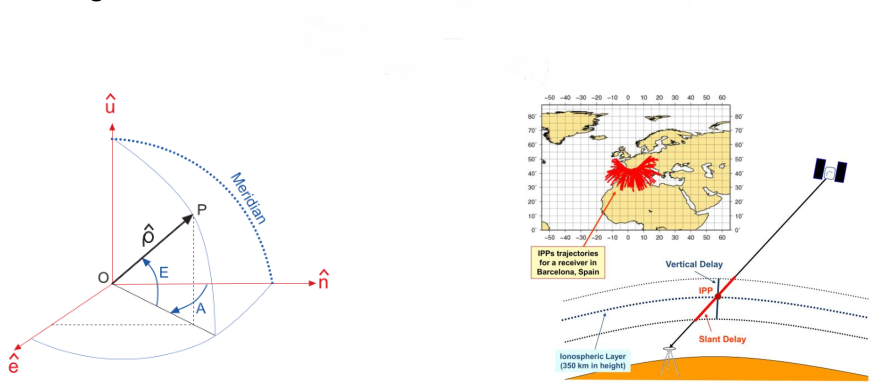
\includegraphics[width=1\textwidth]{elev}
		\caption{Kut elevacije (izvor)}
		\label{fig:elev}
	\end{minipage}
	\begin{minipage}{0.9\textwidth}
		\centering
		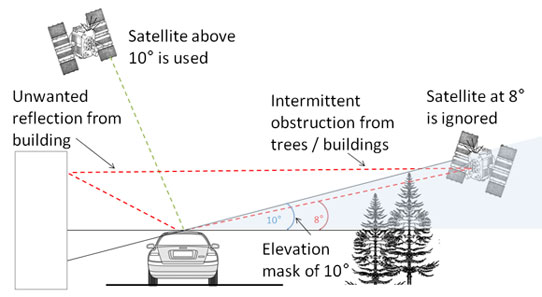
\includegraphics[width=1\textwidth]{elevBetter}
		\caption{Kut elevacije u odnosu na prijemnik u automobilu (\url{https://racelogic.support/01VBOX_Automotive/01VBOX_data_loggers/VBOX_3i_Range/VBOX_3i_User_Manual_(All_Variants)/02_-_VB3i_GPS_Antenna_Placement})}
		\label{fig:elevBetter}
	\end{minipage}
\end{figure}%

Ponovno lineariziramo desne strane jednadžbi \ref{eq:1partial} i dobivamo da $\forall i \in \{1,2,3,4, ...\}$
\begin{align*}
d_i - \sqrt{(x_k-x_i)^{2}+(y_k-y_i)^{2}+(z_k-z_i)^{2}} - c\cdot (d_T)_k & = \\
\frac{\partial f}{\partial x}\Delta x_k + \frac{\partial f}{\partial y}\Delta y_k + \frac{\partial f}{\partial z}\Delta z_k + \frac{\partial f}{\partial d_T}\Delta (d_T)_k &= 
\begin{bmatrix}
\frac{\partial f_i}{\partial x} &
\frac{\partial f_i}{\partial y} &
\frac{\partial f_i}{\partial z} &
\frac{\partial f_i}{\partial d_T}
\end{bmatrix}
\begin{bmatrix}
\Delta x \\
\Delta y \\
\Delta z \\
\Delta d_T
\end{bmatrix} \\ 
\end{align*}
gdje je $i$ indeks pridružen vrijednostima i-te jednadžbe sustava.

Općenito, $i$ može biti proizvoljan. 
Glavno da sadrži najmanje onoliko nezavisnih jednadžbi koliko sustav ima nepoznanica.
Do sada se većinom promatrao sustav $i = 4 = \textit{broj nepoznanica sustava}$ s međusobno nezavisnim jednadžbama. Nastavimo u istom tonu.
\\
Uz 
\begin{align*}
\mathbf{A} & := \begin{bmatrix}
\frac{\partial f_1}{\partial x} &
\frac{\partial f_1}{\partial y} &
\frac{\partial f_1}{\partial z} &
\frac{\partial f_1}{\partial d_T} \\
\frac{\partial f_2}{\partial x} &
\frac{\partial f_2}{\partial y} &
\frac{\partial f_2}{\partial z} &
\frac{\partial f_2}{\partial d_T} \\
\frac{\partial f_3}{\partial x} &
\frac{\partial f_3}{\partial y} &
\frac{\partial f_3}{\partial z} &
\frac{\partial f_3}{\partial d_T} \\
\frac{\partial f_4}{\partial x} &
\frac{\partial f_4}{\partial y} &
\frac{\partial f_4}{\partial z} &
\frac{\partial f_4}{\partial d_T}
\end{bmatrix}  \\
& = \begin{bmatrix}
\frac{(x-x_1)}{\sqrt{(x-x_1)^{2}+(y-y_1)^{2}+(z-z_1)^{2}}} & \frac{(y-y_1)}{\sqrt{(x-x_1)^{2}+(y-y_1)^{2}+(z-z_1)^{2}}} & \frac{(z-z_1)}{\sqrt{(x-x_1)^{2}+(y-y_1)^{2}+(z-z_1)^{2}}} & c \\
\frac{(x-x_2)}{\sqrt{(x-x_2)^{2}+(y-y_2)^{2}+(z-z_2)^{2}}} & \frac{(y-y_2)}{\sqrt{(x-x_2)^{2}+(y-y_2)^{2}+(z-z_2)^{2}}} & \frac{(z-z_2)}{\sqrt{(x-x_2)^{2}+(y-y_2)^{2}+(z-z_2)^{2}}} & c \\
\frac{(x-x_3)}{\sqrt{(x-x_3)^{2}+(y-y_3)^{2}+(z-z_3)^{2}}} & \frac{(y-y_3)}{\sqrt{(x-x_3)^{2}+(y-y_3)^{2}+(z-z_3)^{2}}} & \frac{(z-z_3)}{\sqrt{(x-x_3)^{2}+(y-y_3)^{2}+(z-z_3)^{2}}} & c \\
\frac{(x-x_4)}{\sqrt{(x-x_4)^{2}+(y-y_4)^{2}+(z-z_4)^{2}}} & \frac{(y-y_4)}{\sqrt{(x-x_4)^{2}+(y-y_4)^{2}+(z-z_4)^{2}}} & \frac{(z-z_4)}{\sqrt{(x-x_4)^{2}+(y-y_4)^{2}+(z-z_4)^{2}}} & c \\
\end{bmatrix}\\
\end{align*}
\begin{align}
\mathbf{x} & :=  \begin{bmatrix}
\Delta x \\
\Delta y \\
\Delta z \\
\Delta d_T
\end{bmatrix}\\
\mathbf{b} & := \begin{bmatrix}
d_1 - \sqrt{(x_k-x_1)^{2}+(y_k-y_1)^{2}+(z_k-z_1)^{2}} - c\cdot (d_T)_k \\
d_2 - \sqrt{(x_k-x_2)^{2}+(y_k-y_2)^{2}+(z_k-z_2)^{2}} - c\cdot (d_T)_k \\
d_3 - \sqrt{(x_k-x_3)^{2}+(y_k-y_3)^{2}+(z_k-z_3)^{2}} - c\cdot (d_T)_k \\
d_4 - \sqrt{(x_k-x_4)^{2}+(y_k-y_4)^{2}+(z_k-z_4)^{2}} - c\cdot (d_T)_k
\end{bmatrix}
\end{align}
imamo sustav:
\begin{align*}
\mathbf{A}\mathbf{x} = \mathbf{b}
\end{align*} i
\begin{align*}
\mathbf{p}(\mathbf{x}) := \mathbf{A}\mathbf{x} - \mathbf{b}
\end{align*}


Praksa nerjetko koristi samo jedan signal prilikom postupka procjene položaja i utjecaj ionosfere modelira 
na opisan način.

\subsection{Izvedba }
Prilikom izvedbe algoritma koristimo sustav s $i = 7$ jednadžbi.
Programski isječak koji izvodi opisanu metodu dan je u dodatku \ref{appendix:izvedba}.

Budući da za težine opisane jednadžbom \ref{eq:elevationTezine1} dobivamo,
konvergenciju navedenog algoritma u samo jednom koraku s pogreškom točnosti veličine $10E9$,
uvodimo kut $\psi_0$ koji rješava problem singulariteta funkcije koja opisuje težine.
Dobivamo opis težina sljedećom jednadžbom:
\begin{align}\label{eq:elevationTezine2}
\sigma^2_i = \frac{1}{ \sin ( Ele_i + \psi_0) }
\end{align}
Za $\psi = 0.5$, algoritam konvergira sporije (u 55 koraka) s točnošću $10E3$, očekivane točnosti.

\subsection{Rasprava o kvaliteti}
Uvođenjem težina dobivamo i treći izvedbu algoritma za procjenu položaja u domeni navigacijske primjene. Ovoga puta nije izveden osnovni algoritam, već poboljšani. Uvedene su težine.

Promatrajući njegovu kvalitetu dobivamo sljedeće rezultate:
\begin{table}[H]
	\caption{Kvaliteta druge izvedbe poboljšanog algoritma za procjenu položaja u domani navigacijske primjene}
	%\rowcolors{1}{}{lightgray}
	\begin{center}
		\begin{tabular}{|p{3cm}|p{4cm}}
			\hline
			\rowcolor{lightgray}NAZIV&   \\
			\rowcolor{lightgray}&   \\
			\multirow{-3}{1cm}{ \cellcolor{lightgray}PARAMETRA} & \multirow{-3}{2cm}{\cellcolor{lightgray}VRIJEDNOST} \\
			\hline
			\vspace{0.1cm}
			vrijeme izvršavanja & \vspace{0.1cm}  0.45\\
			\vspace{0.1cm}
			broj iteracija do konvergencije & \vspace{0.1cm} $55$ \\
			\vspace{0.1cm}
			točnost procjene & \vspace{0.1cm} $10^3$ \\
			\hline
		\end{tabular}
	\end{center}
\end{table}

\begin{figure}[H]
	\begin{minipage}{0.48\textwidth}
		\centering
		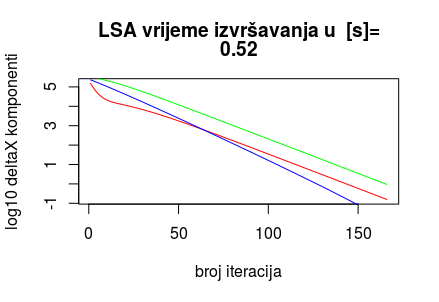
\includegraphics[width=1\textwidth]{3LSAdeltal10}
		\caption{Logaritam vrijednosti $\Delta x$ po komponentama kroz iteracije}
		\label{fig:3LSAdeltal10}
	\end{minipage}%	
	\hspace{1cm}
	\begin{minipage}{0.48\textwidth}
		
		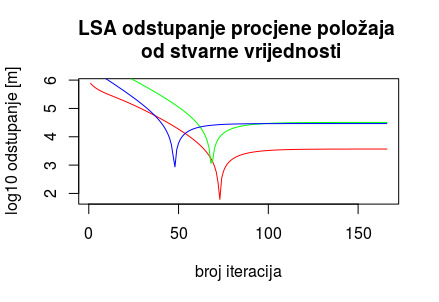
\includegraphics[width=1\textwidth]{3LSAreall10}
		\caption{Logaritam vrijednosti odstupanja od pravog položaja po komponentama kroz iteracije}
		\label{fig:3LSAreall10}
	\end{minipage}%
\end{figure}

Sa slika \ref{fig:3LSAdeltal10} i \ref{fig:3LSAreall10} je vidljivo kako poboljšana treća izvedba
(izvedba algoritma \ref{code:iterLSMW}) dovodi do konvergencije rješenju u okvirima očekivane točnosti.\\



\section{Usporedba osnovnog i poboljšanog algoritma} + zaključak zašto je bolji.
%TEMELJEM ONIH 3 STAVKI
\chapter{Zaključak}
Potrebno promatrati i druge parametre, utjecaje refleksije, ionosfere itd.
%NAPIŠI I BEZ ONIH KVADRIRANJA I SRANJA == kako rademo u baski + vidi zasto te tezine
%; TOJE POČETNI ALG KOJI SMO MODIFICIRALI


%\label{stranica}
%Na stranici \pageref{stranica} se nalaza slika u \textbf{png} formatu.

\bibliographystyle{babamspl} % babamspl ili babplain

% U datoteku diplomski.bib se stavljaju bibliografske reference
% Bibliografske reference u bib formatu se mogu dobiti iz MathSciNet baze, Google Scholara, ArXiva, ...
\bibliography{diplomski}

\pagestyle{empty} % ne zelimo brojanje sljedecih stranica

% I na koncu idu sazeci na hrvatskom i engleskom

\begin{sazetak}
Satelitsko određivanje položja predstavlja temeljnu
tehnologiju rastućeg broja tehnoloških i društveno-ekonomskih sustava.
Kvaliteta njihovih
usluga određena je točnoću procjene položja
satelitskim sustavima.
Programski određen radioprijamnik za satelitsku navigaciju
procesira signale za određivanje položja i podatke
iz navigacijske poruke
u tri osnovne domene: radiofrekvencijskoj, u domeni osnovnog frekvencijskog
područja te u domeni navigacijske primjene.
Ovaj rad analizira postupak procjene položaja
u domeni navigacijske primjene. U tu svrhu, koriste se na osobnom računalu
izveden programski određen GPS prijamnik i ulazni podatci
o opaženim pseudoudaljenostima spremljeni
u RINEX podatkovnom formatu.
Analiza korištenog algoritma procjene položaja
temelji se na izmjerenim pseudoudaljenosti (Sanz Subirana et al, 2013, Chapter 6.1)
te se otkrivaju potencijalne slabosti algoritma
s učincima na točnost procjene položja. Na kraju, predlažu se poboljšanja
algoritma te ih se izvodi u programskom okruženju R. 
Poboljšanja algoritma su vrednovana komparativnom analizom obilježja
poboljšanog i izvornog algoritma.
\end{sazetak}

\begin{summary}
In this ...
\end{summary}

% te zivotopis

\begin{cv}
Dana ...
\end{cv}

\appendix

\chapter{Taylorov red potencija}\label{appendix:aTay}
Primjetimo kako smo na stranici \pageref{stranica:NGLin} pretpostavili
kako će za rezidualnu funkciju $\mathbf{p}(\mathbf{x})$ postojati njezin 
razvoj u Taylorov red oko svake točke $\mathbf{x_k}$. Ipak,
Taylorov red nije definiran za svaku funkciju na $\R^n, n \in \N$.
Prilikom primjene Iterativne metode najmanjih kvadrata, treba zahtjevati da 
funkcija $\mathbf{p}(\mathbf{x})$ i točka $x_k$ zadovoljava uvjete definicije razvoja funkcije u Taylorov red oko točke $x_k$ \cite{math:tay}.
\begin{defn}
	Naka je $f: \mathbf{I} \to \R $ funkcija klase $C^\infty(\mathbf{I})$ definirana
	na otvorenom intervalu $\mathbf{I} \subseteq \R^n$ i neka je $c \in \mathbf{I}$.
	Red potencija
	\begin{align}
	T \left[f,c\right] := \sum_{n=0}^{\infty} \frac{f^{(n)}}{n!} \left(x - c\right)^n
	\end{align}
	nazivamo \textbf{Taylorov red} funkcije $f$ oko točke $c$.
\end{defn}%

Također,
pretpostavlja se kako je 
\begin{align}\label{eg:a1}
	\mathbf{p}(\mathbf{x_{k+1}}+\Delta \mathbf{x}_k) = T \left[\mathbf{p},x_k \right]
\end{align}
što općenito nije točno.
Naime, Taylorov red $T \left[f,c\right] $ funkcije 
$f \in C^\infty(\mathbf{I})$ nužno ne konvergira za svaki $x \not = c, x \in \mathbf{I}$
ili može konvergirati prema nekoj drugoj funkciji.
Uvjete pod kojima zaista vrijedi \ref{eg:a1} opisani su teoremima u nastavku.

\begin{defn}[Analitička funkcija]
	Za $f \in C^\infty(\mathbf{I})$ kažemo da je \textbf{analitička u točki} $c \in \mathbf{I}$ ako njezin Taylorov red:
	\begin{align*}
		T \left[f,c\right] := \sum_{n=0}^{\infty} \frac{f^{(n)}}{n!} \left(x - c\right)^n
	\end{align*}
	
	ima radijus konvergencije $R > 0$ i ako postoji $0 < \delta \leq R$ takav da vrijedi 
	\begin{align*}
	f(x) = T \left[f,c\right] := \sum_{n=0}^{\infty} \frac{f^{(n)}}{n!} \left(x - c\right)^n,
	\forall x \in \left < c-\delta, c+\delta \right > \cap \mathbf{I}
	\end{align*}
	U oznaci: $f \in C^\omega(\mathbf{I})$.
\end{defn}
\begin{thm}\label{thm:konv1}
	Neka je $\sum_{n=0}^{\infty} a_n \left(x - c\right)^n$ red potencija s radijusom konvergencije $R > 0$. Za $\mathbf{I} := \left < c-R, c+R\right >$,
	funkcija $f: \mathbf{I} \to \R$ definirana s 
	\begin{align}
		f(x) := \sum_{n=0}^{\infty} a_n \left(x - c\right)^n
	\end{align}
	je analitička na čitavom $\mathbf{I}$. Nadalje, za svaki $\alpha \in \mathbf{I}$ 
	pripadni Taylorov red
	\begin{align}
		T \left[f,\alpha \right] = \sum_{n=0}^{\infty} \frac{f^{(n)}}{n!} \left(x - \alpha \right)^n
	\end{align}
	ima radijus konvergencije $\rho \leq R - (c - \alpha)$ i vrijedi 
	\begin{align}
	f(x) = T \left[f,\alpha \right] = \sum_{n=0}^{\infty} \frac{f^{(n)}}{n!} \left(x - \alpha \right)^n
	\end{align}
\end{thm}


\begin{thm}\label{thm:konv}
	Naka je $f: \mathbf{I} \to \R $ funkcija klase $C^\infty(\mathbf{I})$ definirana
	na otvorenom intervalu $\mathbf{I} \subseteq \R^n$.
	Tada je $f \in C^\omega(\mathbf{I}$ ako i samo ako za svaki $c \in \mathbf{I}$ postoje
	$\delta > 0$ i konstante $C > 0$ i $ r > 0 $ takve da za sve $n \in \Z_+$ vrijedi:
	\begin{align}
		\left | f^{n}(x)  \leq  C \frac{n!}{r^n}  \right | 
		\forall x \in \mathbf{J} := \left < c-\delta, c+\delta \right > \cap \mathbf{I}
	\end{align}
U tom slučaju $f(x) = T \left[f,c\right](x) $ $
\forall x \in \left < c-r, c+r \right > \cap \mathbf{J}$.
\end{thm}
Za primjenu iterativne metode
najmanjih kvadrata $\mathbf{p}$ mora biti klase $C^\infty(\mathbf{I})$ gdje je $\mathbf{I}$ unija otvorenih okolina oko svih izračinatih $\mathbf{x}_k, k \in \N$, osim zadnjega.
Također, otvorena okolina oko $\mathbf{x}_k$  mora barem sadržavaki otvorenu kuglu $K(\mathbf{x}_k,\Delta \mathbf{x}_k)$ i za $\mathbf{p}$ mora vrijediti teorem \ref{thm:konv1} ili  \ref{thm:konv}.

\chapter{Jakobijeva matrica funkcije $\mathbf{h}$, $J$}
Iz jednakosti \ref{eq:matrix2} i $J = \mathbf{p}(\mathbf{x})$ dobivamo
\begin{align}
J = \frac{\partial \mathbf{h}}{\partial \mathbf{x}}
\end{align}
Za 
\begin{align}
\mathbf{h} (\mathbf{x}) := 
\begin{bmatrix}
||(\mathbf{s}_1-\mathbf{x}_{1:3})|| \\
||(\mathbf{s}_2-\mathbf{x}_{1:3})|| \\
||(\mathbf{s}_3-\mathbf{x}_{1:3})||\\
\end{bmatrix} 
\end{align}
dobivamo
\begin{align}
J = \begin{bmatrix}
\frac{\partial}{\partial \mathbf{x}} ||(s_1-\mathbf{x}_{1:3})|| \\
\frac{\partial}{\partial \mathbf{x}} ||(s_2-\mathbf{x}_{1:3})||\\
\frac{\partial}{\partial \mathbf{x}} ||(s_3-\mathbf{x}_{1:3})|| 
\end{bmatrix}%
= - \begin{bmatrix}
\frac{(s_1-\mathbf{x}_{1:4})^T}{||(s_1-\mathbf{x}_{1:3})||} \\
\frac{(s_2-\mathbf{x}_{1:4})^T}{||(s_1-\mathbf{x}_{1:3})||}\\
\frac{(s_3-\mathbf{x}_{1:4})^T}{||(s_1-\mathbf{x}_{1:3})||} 
\end{bmatrix} = (J_n(1:3,1:3))
\end{align}
uz $\hat{\mathbf{x}} = \mathbf{x}_n$
\chapter{Mjere kvalitete "zviježđa"}\label{appendix:DOP}
Proces određivanja položaja prijemnika je najtočniji ukoliko je međusobni položaj korištenih satelita povoljan.
Međusoban odnos između satelita ovisi o kutu između njih.
Nepovoljan odnos između satelita rezultira skoro pa zavisnim sustavom jednadžbi. 
Što je sustav jednadžbi bliži zavisnome, veća je mogućnost da prilikom procesa određivanja položaja prijemnika sustav zaista i postane zavisan. Zavisnost sustava uzrokovana je pogreškama zaokruživanja. One se mogu smanjiti, ali nikada u potpunosti izbjeći.

Jednim imenom se mjere međusobnog odnosa među satelitima ili mjere kvalitete "zviježđa" nazivaju \textit{degradacija točnosti} (\textbf{DOP}, engl. Dilution of precision).
Niske vrijednosti \textbf{DOP}-a znače povoljan, dok 
visoke vrijednosti znače nepovoljan međusobni položaj satelita.
U nastavku navodimo različite \textbf{DOP} mjere \cite{svd_str15}.
Uz%
\begin{align}
\sigma_{0_prior}^2 & := \frac{\mathbf{p_{prior}}^T \mathbf{W}\mathbf{p_{prior}}}{N-4}\\
\mathbf{p_{prior}} & := (p_1(\mathbf{x_0}),p_2(\mathbf{x_0}),p_3(\mathbf{x_0}),p_4(\mathbf{x_0})) \notag \\
\hat{\sigma}_0^2 & := \frac{\mathbf{\hat{p}}^T \mathbf{W}\mathbf{\hat{p}}}{N - 4}
\end{align}
imamo
\begin{align}
\mathbf{Q_{\hat{x}}} & := \hat{\sigma}_0^2(\mathbf{A^1}^T\mathbf{W}\mathbf{A^1})^{-1} \\
\mathbf{Q_{DOP}} & := \frac{\mathbf{Q_{\hat{x}}}}{\hat{\sigma}_0^2 \sigma_{0_prior}^2} \\
& = \frac{(\mathbf{A^1}^T\mathbf{W}\mathbf{A^1})^{-1}}{\sigma_{0_prior}^2} \\
& = \begin{bmatrix}
q_X^2 & q_{YX} & q_{ZX} & q_{d_TX} \\
q_{XY} & q_Y^2 & q_{ZY} & q_{cd_TY} \\
q_{XZ} & q_{YZ} & q_Z^2 & q_{cd_TZ} \\
q_{Xcd_T} & q_{Ycd_T} & q_{Zcd_T} & q_{cd_T}^2 
\end{bmatrix}\\
\mathbf{A^1} & := \begin{bmatrix}
\mathbf{A}[1:N,1:3] & [1 1 1 1]^T
\end{bmatrix}
\end{align}
Prostorna degradacija točnosti određivanja položaja (PDOP, engl. position DOP) je određena izrazom
\begin{align}
PDOP = \sqrt{q_X^2+q_y^2+q_Z^2}
\end{align}
Degradacija točnosti određivanaj vremena (TDOP, engl. time DOP) je određena izrazom
\begin{align}
TDOP = \sqrt{q_{cd_T}^2}
\end{align}
\textbf{DOP} formulacija koja objedunjuje prethodne je geometrijska defradacija točnosti (GDOP, engl. geometric DOP) određena izrazom
\begin{align}
GDOP = \sqrt{q_X^2+q_y^2+q_Z^2+q_{cd_T}^2}
\end{align}
U praksi najčešće promatramo  vrijednosti $PDOP$-a. Vrijednosti $PDOP$-a ispod 2 se smatraju odličnima, između 2 i 4 dobrima, a do 6 prihvatljivima. Vrijednosti iznad 6 su neprihvatljive i sugeriraju nepogodan međusoban položaj satelita.

Dalje definiramo $HDOP$ i $VDOP$. \\
Nakon transformacije gornje lijeve podmatrice matrice $\mathbf{Q-{\hat{x}}}$ veličine $3 \times 3$ iz ECEF XYZ koordinata u ENU koordinate u odnosu na poziciju prijemnika, dobivano matricu $\mathbf{Q}_{ENU}$.
\begin{align}
\mathbf{Q}_{DOP,ENU} & := \frac{\mathbf{Q}_{ENU}}{\hat{\sigma}_0^2 \sigma_{0_prior}^2} \\
&=\begin{bmatrix}
q_E^2 & q_{NE} & q_{UE} \\
q_{EN} & q_{N}^2 & q_{UN} \\
q_{EU}^2 & q_{NU} & q_{U}^2 \\
\end{bmatrix}\\
HDOP & := \sqrt{q_E^2 + q_{N}} \\
VDOP & := \sqrt{q_U^2}
EDOP & := \sqrt{q_E^2 + q_{N}} \\
NDOP & := \sqrt{q_U^2}
\end{align}
gdje $HDOP$ i $VDOP$ nazivamo horizontalna i vertikalna degradacija točnosti, a
$EDOP$ i $NDOP$ su degradacija točnosti u smeru istoka, odnosno sjevera.

\chapter{Kodovi izvedbe algoritama}\label{appendix:izvedba}
\section{Osnovni pristup}
\subsection{Prvi način linearizacije}
\lstinputlisting[language=R]{Rsimulation/dipl2.R}%dipl2.R
\subsection{Drugi način linearizacije}
\lstinputlisting[language=R]{Rsimulation/dipl1.R}%dipl1.R
\section{Poboljšan pristup: uvođenje težina (WLSM)}
\lstinputlisting[language=R]{Rsimulation/dipl4.R}%dipl4.R

\end{document}